\subsection{Small CNNs: performance, fairness and clustering quality}\label{sec:small}
\paragraph{Main results.}
Table~\ref{tab:main} reports Fashion-MNIST results for all methods with five seeds: means with 95\% $t$-intervals over seeds. Accuracy is \emph{with} the prior correction~\eqref{eq:pc}, applied identically to every method. Table~\ref{tab:failure} gives failure rates, Table~\ref{tab:hier} the hierarchical comparison over scenarios, and Table~\ref{tab:diag} the separation and coverage diagnostics of Section~\ref{sec:theory} for every scenario.

\begin{tableorg}[!htbp]
\centering
\caption{Fashion-MNIST, 40 clients, 5 seeds: mean $\pm$ half-width of the 95\% $t$-interval over seeds. Acc: mean local accuracy with prior correction. Concept: accuracy on the class-balanced test set of the client's concept. Worst-grp: accuracy of the worst concept group. Conflict: fraction of conflicting client pairs placed in one cluster. IFCA, FeSEM, FL+HC, PACFL and FedDAG-C receive the true $K$ (in \emph{Label skew only}, $K=1$); DisCo-CFL, MTCFL, StoCFL and FedCCFA find it. For FedCCFA, ARI and $K$ refer to the client partition induced by its per-class clusters.}\label{tab:main}
{\scriptsize
\resizebox{\textwidth}{!}{%
\begin{tabular}{l r c c c c c c}
\toprule
Method & n & Acc (\%) & Concept (\%) & Worst-grp (\%) & ARI & K & Conflict (\%) \\
\midrule
\multicolumn{8}{l}{\textit{Rotation}} \\
DisCo & 5 & 89.1 $\pm$ 1.1 & 76.4 $\pm$ 1.0 & 87.4 $\pm$ 1.7 & 0.92 $\pm$ 0.06 & 4.4 & 1.1 \\
DisCo-noAttach & 5 & 89.1 $\pm$ 1.1 & 76.2 $\pm$ 1.0 & 87.3 $\pm$ 1.6 & 0.91 $\pm$ 0.07 & 4.8 & 1.1 \\
FedAvg & 5 & 82.4 $\pm$ 1.2 & 65.4 $\pm$ 1.1 & 80.7 $\pm$ 2.1 & 0.00 $\pm$ 0.00 & 1.0 & 100.0 \\
Local & 5 & 87.4 $\pm$ 0.9 & 54.0 $\pm$ 2.4 & 85.2 $\pm$ 1.5 & 0.00 $\pm$ 0.00 & 40.0 & 0.0 \\
FedAvg-FT & 5 & 83.7 $\pm$ 1.8 & 64.8 $\pm$ 1.3 & 81.5 $\pm$ 3.2 & 0.00 $\pm$ 0.00 & 40.0 & 0.0 \\
IFCA & 5 & 86.2 $\pm$ 1.9 & 66.9 $\pm$ 4.8 & 84.2 $\pm$ 2.8 & 0.27 $\pm$ 0.21 & 4.0 & 23.6 \\
FeSEM & 5 & 87.4 $\pm$ 1.7 & 70.8 $\pm$ 3.4 & 85.8 $\pm$ 1.5 & 0.43 $\pm$ 0.28 & 4.0 & 24.7 \\
MTCFL & 5 & 88.1 $\pm$ 1.3 & 64.1 $\pm$ 2.2 & 86.8 $\pm$ 1.5 & 0.11 $\pm$ 0.02 & 24.2 & 0.3 \\
FL+HC & 5 & 88.4 $\pm$ 0.9 & 74.3 $\pm$ 2.2 & 86.9 $\pm$ 0.8 & 0.70 $\pm$ 0.18 & 4.0 & 9.3 \\
PACFL & 5 & 87.5 $\pm$ 1.6 & 72.0 $\pm$ 1.0 & 85.2 $\pm$ 2.2 & 0.47 $\pm$ 0.09 & 4.0 & 20.6 \\
StoCFL & 5 & 85.3 $\pm$ 1.6 & 61.2 $\pm$ 1.5 & 83.1 $\pm$ 1.4 & 0.03 $\pm$ 0.06 & 12.6 & 8.6 \\
StoCFL-W & 5 & 86.7 $\pm$ 1.3 & 64.8 $\pm$ 2.1 & 84.9 $\pm$ 1.4 & 0.10 $\pm$ 0.05 & 16.2 & 3.9 \\
FedCCFA & 5 & 83.3 $\pm$ 0.9 & 62.5 $\pm$ 1.4 & 80.2 $\pm$ 1.1 & 0.00 $\pm$ 0.00 & 1.2 & 99.0 \\
FedDAG-C & 5 & 88.6 $\pm$ 0.7 & 74.2 $\pm$ 3.4 & 86.6 $\pm$ 1.7 & 0.69 $\pm$ 0.26 & 4.0 & 12.1 \\
Oracle & 5 & 89.3 $\pm$ 1.0 & 77.4 $\pm$ 0.7 & 87.6 $\pm$ 1.6 & 1.00 $\pm$ 0.00 & 4.0 & 0.0 \\
\addlinespace
\multicolumn{8}{l}{\textit{Label swap}} \\
DisCo & 5 & 89.2 $\pm$ 0.9 & 76.7 $\pm$ 0.8 & 87.7 $\pm$ 1.1 & 0.97 $\pm$ 0.05 & 4.0 & 0.0 \\
DisCo-noAttach & 5 & 89.2 $\pm$ 0.9 & 76.5 $\pm$ 1.0 & 87.7 $\pm$ 1.1 & 0.97 $\pm$ 0.04 & 4.2 & 0.0 \\
FedAvg & 5 & 74.7 $\pm$ 2.7 & 53.3 $\pm$ 0.5 & 67.1 $\pm$ 6.7 & 0.00 $\pm$ 0.00 & 1.0 & 100.0 \\
Local & 5 & 87.3 $\pm$ 1.0 & 54.2 $\pm$ 2.3 & 85.3 $\pm$ 1.3 & 0.00 $\pm$ 0.00 & 40.0 & 0.0 \\
FedAvg-FT & 5 & 85.5 $\pm$ 2.2 & 66.3 $\pm$ 1.5 & 83.4 $\pm$ 2.8 & 0.00 $\pm$ 0.00 & 40.0 & 0.0 \\
IFCA & 5 & 84.5 $\pm$ 1.9 & 61.2 $\pm$ 7.2 & 82.1 $\pm$ 2.7 & 0.30 $\pm$ 0.15 & 4.0 & 19.7 \\
FeSEM & 5 & 85.8 $\pm$ 1.7 & 64.8 $\pm$ 5.8 & 81.3 $\pm$ 4.6 & 0.39 $\pm$ 0.13 & 4.0 & 17.9 \\
MTCFL & 5 & 88.1 $\pm$ 1.3 & 64.4 $\pm$ 2.8 & 86.2 $\pm$ 1.1 & 0.11 $\pm$ 0.02 & 24.2 & 0.1 \\
FL+HC & 5 & 88.3 $\pm$ 0.9 & 72.6 $\pm$ 4.4 & 86.5 $\pm$ 2.0 & 0.69 $\pm$ 0.31 & 4.0 & 7.7 \\
PACFL & 5 & 76.8 $\pm$ 3.9 & 50.6 $\pm$ 1.3 & 70.5 $\pm$ 5.2 & $-$0.02 $\pm$ 0.02 & 4.0 & 35.1 \\
StoCFL & 5 & 81.3 $\pm$ 2.7 & 53.2 $\pm$ 1.8 & 74.9 $\pm$ 6.8 & 0.01 $\pm$ 0.04 & 11.4 & 9.5 \\
StoCFL-W & 5 & 86.8 $\pm$ 1.5 & 64.1 $\pm$ 2.6 & 85.0 $\pm$ 1.0 & 0.15 $\pm$ 0.04 & 16.4 & 3.2 \\
FedCCFA & 5 & 85.7 $\pm$ 0.7 & 64.3 $\pm$ 1.5 & 82.4 $\pm$ 2.3 & 0.00 $\pm$ 0.00 & 2.4 & 92.7 \\
FedDAG-C & 5 & 84.2 $\pm$ 2.9 & 61.7 $\pm$ 4.3 & 80.6 $\pm$ 3.9 & 0.37 $\pm$ 0.14 & 4.0 & 21.1 \\
Oracle & 5 & 89.2 $\pm$ 1.0 & 77.0 $\pm$ 0.8 & 87.7 $\pm$ 1.3 & 1.00 $\pm$ 0.00 & 4.0 & 0.0 \\
\addlinespace
\multicolumn{8}{l}{\textit{Rotation + QS}} \\
DisCo & 5 & 88.9 $\pm$ 2.5 & 76.4 $\pm$ 1.5 & 86.5 $\pm$ 4.0 & 0.99 $\pm$ 0.03 & 4.2 & 0.0 \\
DisCo-noAttach & 5 & 88.8 $\pm$ 2.4 & 76.1 $\pm$ 1.6 & 86.2 $\pm$ 3.5 & 0.97 $\pm$ 0.05 & 4.8 & 0.0 \\
FedAvg & 5 & 81.6 $\pm$ 4.2 & 62.7 $\pm$ 4.5 & 75.3 $\pm$ 10.0 & 0.00 $\pm$ 0.00 & 1.0 & 100.0 \\
Local & 5 & 85.3 $\pm$ 2.7 & 51.9 $\pm$ 2.0 & 81.8 $\pm$ 5.3 & 0.00 $\pm$ 0.00 & 40.0 & 0.0 \\
FedAvg-FT & 5 & 82.2 $\pm$ 1.7 & 62.8 $\pm$ 2.6 & 77.9 $\pm$ 4.0 & 0.00 $\pm$ 0.00 & 40.0 & 0.0 \\
IFCA & 5 & 87.6 $\pm$ 2.1 & 71.5 $\pm$ 1.9 & 84.5 $\pm$ 3.9 & 0.54 $\pm$ 0.19 & 3.8 & 17.7 \\
FeSEM & 5 & 83.0 $\pm$ 2.1 & 64.3 $\pm$ 4.4 & 76.7 $\pm$ 5.2 & 0.22 $\pm$ 0.18 & 4.0 & 36.8 \\
MTCFL & 5 & 87.0 $\pm$ 2.4 & 63.4 $\pm$ 2.2 & 84.1 $\pm$ 4.1 & 0.11 $\pm$ 0.01 & 24.8 & 0.2 \\
FL+HC & 5 & 86.5 $\pm$ 2.7 & 71.2 $\pm$ 2.7 & 83.6 $\pm$ 2.7 & 0.56 $\pm$ 0.22 & 4.0 & 17.6 \\
PACFL & 5 & 85.8 $\pm$ 3.8 & 69.7 $\pm$ 5.5 & 81.4 $\pm$ 7.3 & 0.44 $\pm$ 0.05 & 4.0 & 21.9 \\
StoCFL & 5 & 83.5 $\pm$ 1.7 & 59.4 $\pm$ 2.4 & 80.7 $\pm$ 2.8 & 0.05 $\pm$ 0.07 & 14.0 & 7.4 \\
StoCFL-W & 5 & 85.8 $\pm$ 2.8 & 65.0 $\pm$ 2.5 & 82.6 $\pm$ 4.8 & 0.17 $\pm$ 0.09 & 17.2 & 3.7 \\
FedCCFA & 5 & 83.4 $\pm$ 3.4 & 61.0 $\pm$ 2.6 & 78.8 $\pm$ 8.3 & 0.00 $\pm$ 0.00 & 1.2 & 99.0 \\
FedDAG-C & 5 & 86.3 $\pm$ 2.8 & 69.1 $\pm$ 1.8 & 82.5 $\pm$ 5.2 & 0.44 $\pm$ 0.07 & 4.0 & 19.6 \\
Oracle & 5 & 88.9 $\pm$ 2.5 & 76.7 $\pm$ 2.0 & 86.6 $\pm$ 4.0 & 1.00 $\pm$ 0.00 & 4.0 & 0.0 \\
\addlinespace
\bottomrule
\end{tabular}}
}


\end{tableorg}

\begin{tableorg}[!htbp]
\centering
\noindent\textit{Table~\ref{tab:main} (continued).}\par\smallskip
{\scriptsize
\resizebox{\textwidth}{!}{%
\begin{tabular}{l r c c c c c c}
\toprule
Method & n & Acc (\%) & Concept (\%) & Worst-grp (\%) & ARI & K & Conflict (\%) \\
\midrule
\multicolumn{8}{l}{\textit{Mixed + QS}} \\
DisCo & 5 & 89.0 $\pm$ 2.6 & 76.4 $\pm$ 1.3 & 86.7 $\pm$ 4.1 & 0.96 $\pm$ 0.07 & 4.2 & 0.0 \\
DisCo-noAttach & 5 & 89.0 $\pm$ 2.5 & 76.2 $\pm$ 1.5 & 86.7 $\pm$ 3.9 & 0.96 $\pm$ 0.07 & 4.4 & 0.0 \\
FedAvg & 5 & 81.8 $\pm$ 3.4 & 61.3 $\pm$ 1.3 & 75.0 $\pm$ 6.8 & 0.00 $\pm$ 0.00 & 1.0 & 100.0 \\
Local & 5 & 85.4 $\pm$ 2.8 & 51.8 $\pm$ 1.7 & 81.9 $\pm$ 4.8 & 0.00 $\pm$ 0.00 & 40.0 & 0.0 \\
FedAvg-FT & 5 & 84.0 $\pm$ 1.1 & 66.2 $\pm$ 1.6 & 81.1 $\pm$ 1.7 & 0.00 $\pm$ 0.00 & 40.0 & 0.0 \\
IFCA & 5 & 87.6 $\pm$ 2.1 & 71.2 $\pm$ 0.7 & 85.0 $\pm$ 4.0 & 0.49 $\pm$ 0.09 & 3.6 & 23.3 \\
FeSEM & 5 & 83.3 $\pm$ 2.0 & 63.5 $\pm$ 2.9 & 76.9 $\pm$ 3.3 & 0.11 $\pm$ 0.09 & 4.0 & 40.3 \\
MTCFL & 5 & 87.7 $\pm$ 1.6 & 63.4 $\pm$ 2.3 & 85.7 $\pm$ 2.6 & 0.08 $\pm$ 0.03 & 25.6 & 0.6 \\
FL+HC & 5 & 84.8 $\pm$ 4.0 & 66.8 $\pm$ 1.8 & 80.6 $\pm$ 6.4 & 0.24 $\pm$ 0.13 & 4.0 & 30.3 \\
PACFL & 5 & 82.5 $\pm$ 3.3 & 61.2 $\pm$ 2.4 & 78.6 $\pm$ 4.2 & 0.19 $\pm$ 0.12 & 4.0 & 22.8 \\
StoCFL & 5 & 83.1 $\pm$ 2.2 & 61.1 $\pm$ 1.4 & 79.2 $\pm$ 3.2 & 0.03 $\pm$ 0.06 & 12.2 & 8.6 \\
StoCFL-W & 5 & 85.3 $\pm$ 2.2 & 63.5 $\pm$ 1.5 & 81.0 $\pm$ 4.3 & 0.08 $\pm$ 0.06 & 14.8 & 5.7 \\
FedCCFA & 5 & 85.6 $\pm$ 2.3 & 65.5 $\pm$ 2.1 & 81.8 $\pm$ 3.5 & 0.00 $\pm$ 0.00 & 1.2 & 98.9 \\
FedDAG-C & 5 & 82.2 $\pm$ 3.0 & 60.1 $\pm$ 2.4 & 77.4 $\pm$ 3.3 & 0.20 $\pm$ 0.20 & 4.0 & 31.9 \\
Oracle & 5 & 89.1 $\pm$ 2.4 & 76.8 $\pm$ 1.7 & 86.7 $\pm$ 4.1 & 1.00 $\pm$ 0.00 & 4.0 & 0.0 \\
\addlinespace
\multicolumn{8}{l}{\textit{Label skew only}} \\
DisCo & 5 & 94.5 $\pm$ 1.0 & 76.7 $\pm$ 2.0 & 94.5 $\pm$ 1.0 & 1.00 $\pm$ 0.00 & 1.0 & 0.0 \\
DisCo-noAttach & 5 & 94.5 $\pm$ 1.0 & 76.5 $\pm$ 1.5 & 94.5 $\pm$ 1.0 & 0.80 $\pm$ 0.56 & 1.2 & 0.0 \\
FedAvg & 5 & 94.5 $\pm$ 1.0 & 76.7 $\pm$ 2.0 & 94.5 $\pm$ 1.0 & 1.00 $\pm$ 0.00 & 1.0 & 0.0 \\
Local & 5 & 92.4 $\pm$ 2.2 & 35.4 $\pm$ 0.9 & 92.4 $\pm$ 2.2 & 0.00 $\pm$ 0.00 & 40.0 & 0.0 \\
FedAvg-FT & 5 & 91.6 $\pm$ 2.0 & 71.0 $\pm$ 2.1 & 91.6 $\pm$ 2.0 & 0.00 $\pm$ 0.00 & 40.0 & 0.0 \\
IFCA & 5 & 94.5 $\pm$ 1.2 & 76.4 $\pm$ 2.0 & 94.5 $\pm$ 1.2 & 1.00 $\pm$ 0.00 & 1.0 & 0.0 \\
FeSEM & 5 & 94.6 $\pm$ 1.0 & 76.7 $\pm$ 2.2 & 94.6 $\pm$ 1.0 & 1.00 $\pm$ 0.00 & 1.0 & 0.0 \\
MTCFL & 5 & 93.7 $\pm$ 1.2 & 54.8 $\pm$ 4.5 & 93.7 $\pm$ 1.2 & 0.00 $\pm$ 0.00 & 26.4 & 0.0 \\
FL+HC & 5 & 94.5 $\pm$ 1.0 & 76.6 $\pm$ 1.9 & 94.5 $\pm$ 1.0 & 1.00 $\pm$ 0.00 & 1.0 & 0.0 \\
PACFL & 5 & 94.5 $\pm$ 1.0 & 76.7 $\pm$ 2.0 & 94.5 $\pm$ 1.0 & 1.00 $\pm$ 0.00 & 1.0 & 0.0 \\
StoCFL & 5 & 93.5 $\pm$ 1.4 & 68.6 $\pm$ 1.6 & 93.5 $\pm$ 1.4 & 0.00 $\pm$ 0.00 & 9.6 & 0.0 \\
StoCFL-W & 5 & 93.4 $\pm$ 1.1 & 70.7 $\pm$ 2.0 & 93.4 $\pm$ 1.1 & 0.00 $\pm$ 0.00 & 9.4 & 0.0 \\
FedCCFA & 5 & 93.1 $\pm$ 1.5 & 71.9 $\pm$ 2.5 & 93.1 $\pm$ 1.5 & 1.00 $\pm$ 0.00 & 1.0 & 0.0 \\
FedDAG-C & 5 & 94.5 $\pm$ 1.1 & 76.7 $\pm$ 1.9 & 94.5 $\pm$ 1.1 & 1.00 $\pm$ 0.00 & 1.0 & 0.0 \\
Oracle & 5 & 94.5 $\pm$ 1.0 & 76.7 $\pm$ 2.0 & 94.5 $\pm$ 1.0 & 1.00 $\pm$ 0.00 & 1.0 & 0.0 \\
\addlinespace
\multicolumn{8}{l}{\textit{Minority groups}} \\
DisCo & 5 & 89.2 $\pm$ 0.9 & 77.2 $\pm$ 1.2 & 87.2 $\pm$ 1.0 & 0.99 $\pm$ 0.01 & 4.0 & 0.1 \\
DisCo-noAttach & 5 & 89.2 $\pm$ 0.9 & 77.1 $\pm$ 1.4 & 87.1 $\pm$ 0.8 & 0.97 $\pm$ 0.07 & 4.6 & 0.0 \\
FedAvg & 5 & 83.4 $\pm$ 1.2 & 67.0 $\pm$ 0.8 & 67.5 $\pm$ 11.8 & 0.00 $\pm$ 0.00 & 1.0 & 100.0 \\
Local & 5 & 87.5 $\pm$ 0.9 & 54.2 $\pm$ 2.3 & 86.0 $\pm$ 1.2 & 0.00 $\pm$ 0.00 & 40.0 & 0.0 \\
FedAvg-FT & 5 & 85.0 $\pm$ 1.9 & 66.9 $\pm$ 0.6 & 78.8 $\pm$ 5.7 & 0.00 $\pm$ 0.00 & 40.0 & 0.0 \\
IFCA & 5 & 87.0 $\pm$ 1.2 & 70.0 $\pm$ 4.1 & 81.2 $\pm$ 3.4 & 0.37 $\pm$ 0.31 & 4.0 & 17.8 \\
FeSEM & 5 & 87.7 $\pm$ 1.9 & 72.2 $\pm$ 3.1 & 80.9 $\pm$ 7.8 & 0.47 $\pm$ 0.32 & 4.0 & 14.7 \\
MTCFL & 5 & 88.3 $\pm$ 0.8 & 65.7 $\pm$ 1.1 & 85.7 $\pm$ 2.2 & 0.05 $\pm$ 0.01 & 24.4 & 0.1 \\
FL+HC & 5 & 88.6 $\pm$ 1.4 & 74.4 $\pm$ 0.8 & 83.8 $\pm$ 2.1 & 0.66 $\pm$ 0.20 & 4.0 & 8.6 \\
PACFL & 5 & 88.0 $\pm$ 0.8 & 72.6 $\pm$ 1.8 & 84.2 $\pm$ 1.2 & 0.45 $\pm$ 0.07 & 4.0 & 18.3 \\
StoCFL & 5 & 86.5 $\pm$ 1.3 & 65.4 $\pm$ 0.8 & 83.3 $\pm$ 1.7 & 0.03 $\pm$ 0.05 & 12.4 & 8.3 \\
StoCFL-W & 5 & 87.4 $\pm$ 0.8 & 67.8 $\pm$ 1.3 & 84.6 $\pm$ 1.9 & 0.07 $\pm$ 0.02 & 15.6 & 3.6 \\
FedCCFA & 5 & 84.7 $\pm$ 1.5 & 64.9 $\pm$ 1.0 & 75.5 $\pm$ 8.8 & 0.01 $\pm$ 0.04 & 1.2 & 98.3 \\
FedDAG-C & 5 & 88.5 $\pm$ 1.0 & 74.1 $\pm$ 2.4 & 84.1 $\pm$ 3.6 & 0.68 $\pm$ 0.27 & 4.0 & 11.7 \\
Oracle & 5 & 89.3 $\pm$ 0.8 & 77.3 $\pm$ 1.2 & 87.4 $\pm$ 1.0 & 1.00 $\pm$ 0.00 & 4.0 & 0.0 \\
\bottomrule
\end{tabular}}
}


\end{tableorg}

\paragraph{Recovery of the concept groups (H2).} In all six Fashion-MNIST scenarios DisCo-CFL recovers the groups without being told $K$: mean ARI $0.92$--$1.00$, at most $1.1\%$ of the conflicting pairs merged, and no run with ARI below $0.5$ (Table~\ref{tab:failure}). The weakest scenario is \emph{Rotation} (ARI $0.92\pm0.06$, $K=4.4$): the $0^\circ$ and $180^\circ$ groups are close on the nearly symmetric classes, and some clients that hold mostly such classes are split off or merged. The diagnostics agree with the assumptions of Theorem~\ref{thm:rec}: the estimated separation is $\hat\Delta=0.44$--$0.61$, well above $1-\tau=0.1$, and $94$--$100\%$ of the conflicting pairs share a discriminative class (Table~\ref{tab:diag}). Accuracy and worst-group accuracy are within $0.2$ points of the Oracle in every scenario, and concept accuracy within $1.0$ point.

The baselines that are given the true $K$ merge many conflicting pairs: IFCA 18--24\%, FeSEM 15--40\%, PACFL 18--35\%, FedDAG-C 12--32\% and FL+HC 8--30\%, and they fail (ARI $<0.5$) in 36--88\% of the runs. The closest methods do not recover the groups either. StoCFL compares whole-model gradients at the initial model and fragments the federation into 11--14 clusters with ARI at most $0.05$; with gradients at the warm-up model (StoCFL-W) it forms 15--17 clusters, ARI $\le0.17$. The raw gradient mixes the concept with each client's label mix, exactly the entanglement that the class-conditional signature removes. FedCCFA clusters the classifier of each class separately; its per-class clusters rarely differ between concept groups at the published radius, so the induced partition is almost a single cluster (ARI $0.00$) and its accuracy is 3--6 points below DisCo-CFL. FedDAG-C, which also compares clients class by class but uses data subspaces and gradient angles, is the strongest new baseline on \emph{Rotation} (ARI $0.69$) and much weaker on label swaps (ARI $0.37$), where the data subspaces do not change.

\paragraph{Label skew does not create clusters (H1).} With a single concept and strong target and quantity skew (\emph{Label skew only}), DisCo-CFL returns $K=1$ in all five seeds, and its accuracy equals FedAvg's. MTCFL splits the federation into 26 clusters, StoCFL and StoCFL-W into 9--10, and their concept accuracy drops by 6--22 points. The baselines that receive $K$ are given $K=1$ here, so their single cluster is not a decision.

\paragraph{Performance.} DisCo-CFL is within the confidence interval of the Oracle in every Fashion-MNIST scenario. Its mean accuracy is the highest of all non-oracle methods in the five concept-shift scenarios; in \emph{Label skew only} it equals FedAvg's, and FeSEM is $0.1$ points higher. The margins over the strongest baseline are small on local accuracy (0.5--1.3 points against FedDAG-C, FL+HC, IFCA or MTCFL) and larger on concept accuracy (2.1--5.2 points). Methods that fragment the federation (Local, FedAvg-FT, MTCFL) obtain competitive \emph{local} accuracy, because local test sets share the client's label mix, but their concept accuracy is 10--22 points lower: their models do not generalise to the rest of the client's concept. Across all small-CNN scenarios, the hierarchical bootstrap gives DisCo-CFL a positive mean advantage over every baseline, with 95\% intervals that exclude zero (Table~\ref{tab:hier}); the smallest is $+1.5$ points against FL+HC.

\paragraph{Prior correction and clustering are separate effects.} Table~\ref{tab:decomp} evaluates every method with and without the prior correction. On Fashion-MNIST the correction adds 10--16 points to every method that shares models across clients and 1--4 points to the fragmenting ones (MTCFL, StoCFL); it adds $10.8$ points to DisCo-CFL and $10.9$ to the Oracle. Without the correction DisCo-CFL is $12$ points above FedAvg (79.2\% against 66.8\%) and as accurate as the Oracle; with it, the gap to FedAvg is $7$ points. The correction therefore does not explain the advantage of DisCo-CFL over the other clustering methods, which all receive it; it explains why concept-level clustering, which deliberately keeps clients with different label mixes together, is competitive on local metrics.

\paragraph{Attachment.} Post-processing rarely acts: on Fashion-MNIST it attaches 0.2--0.6 clients per run, and it never created a conflicting pair except in \emph{Minority groups} (0.1\% of the conflicting pairs). DisCo-noAttach has the same accuracy within $0.1$ points. The attachment stage matters in \emph{Label skew only}, where without it a client with a noisy signature stays alone in one seed out of five (ARI $0.80$ instead of $1.00$).

\paragraph{Fairness.} DisCo-CFL has the highest worst-group accuracy among non-oracle methods in all concept-shift scenarios. The gap is largest for minority concepts: in \emph{Minority groups} (25/9/4/2 clients) the worst group reaches 87.2\% with DisCo-CFL, against 67.5\% with FedAvg, 75.5\% with FedCCFA, 80.9--81.2\% with FeSEM and IFCA, and 83.8--84.2\% with FL+HC, PACFL and FedDAG-C. Table~\ref{tab:minority} isolates the clustering step: DisCo-CFL recovers minority groups of 1, 2, 3 and 5 clients with recall and purity $1.00$ and no conflicting merge. FL+HC, which is given $K$, recovers a single-client minority in none of the seeds and merges 8--10\% of the conflicting pairs; PACFL does not find the minority.

\begin{table}[!htbp]
\centering
\caption{Minority-group recovery (clustering step only; groups of 20/10/10/$m$ clients; 3 seeds).}\label{tab:minority}
\small
\begin{tabular}{lcccccc}
\toprule
& \multicolumn{3}{c}{DisCo-CFL} & \multicolumn{3}{c}{FL+HC ($K$ given)} \\
\cmidrule(lr){2-4}\cmidrule(lr){5-7}
$m$ & recall & ARI & conflict\% & recall & ARI & conflict\% \\
\midrule
1 & 1.00 & 1.00 & 0.0 & 0.00 & 0.64 & 10.4\\
2 & 1.00 & 1.00 & 0.0 & 0.33 & 0.73 & 8.5\\
3 & 1.00 & 1.00 & 0.0 & 0.89 & 0.81 & 9.1\\
5 & 1.00 & 1.00 & 0.0 & 0.67 & 0.71 & 8.6\\
\bottomrule
\end{tabular}
\end{table}

\begin{tableorg}[!htbp]
\centering
\caption{Failure rates: fraction of runs with ARI below $0.5$ in scenarios with more than one group (number of runs in parentheses). Main: the five Fashion-MNIST concept-shift scenarios; Other: MNIST, SVHN, CIFAR-10; Sweep: the robustness sweeps; Real: PACS, Office-Home, CIFAR-100.}\label{tab:failure}
{\scriptsize
\begin{tabular}{l c c c c c}
\toprule
Method & Main & Other & Sweep & Real & Extra \\
\midrule
DisCo & 0.0\% (25) & 66.7\% (30) & 4.2\% (24) & 40.0\% (25) & 22.9\% (35) \\
DisCo-noAttach & 0.0\% (25) & 66.7\% (30) & -- & 40.0\% (25) & 25.7\% (35) \\
IFCA & 80.0\% (25) & 80.0\% (30) & 79.2\% (24) & 96.0\% (25) & 71.4\% (35) \\
FeSEM & 76.0\% (25) & 90.0\% (30) & 91.7\% (24) & 100.0\% (25) & 77.1\% (35) \\
MTCFL & 100.0\% (25) & 100.0\% (30) & 100.0\% (24) & 100.0\% (25) & 100.0\% (35) \\
FL+HC & 36.0\% (25) & 73.3\% (30) & 37.5\% (24) & 72.0\% (25) & 54.3\% (35) \\
PACFL & 88.0\% (25) & 96.7\% (30) & 54.2\% (24) & 92.0\% (25) & 90.0\% (30) \\
StoCFL & 100.0\% (25) & 100.0\% (30) & 100.0\% (24) & 100.0\% (25) & 100.0\% (35) \\
StoCFL-W & 100.0\% (25) & 100.0\% (30) & 100.0\% (24) & 100.0\% (25) & 100.0\% (35) \\
FedCCFA & 100.0\% (25) & 100.0\% (30) & 100.0\% (24) & 100.0\% (25) & 94.3\% (35) \\
FedDAG-C & 64.0\% (25) & 86.7\% (30) & 50.0\% (24) & 100.0\% (25) & 66.7\% (30) \\
\bottomrule
\end{tabular}
}

\end{tableorg}

\begin{tableorg}[!htbp]
\centering
\caption{Hierarchical comparison of DisCo-CFL with each baseline (percentage points). $\Delta$: mean difference with a 95\% hierarchical-bootstrap interval (scenarios, then seeds within scenarios; $10^4$ replicates). W/T/L and $p$: wins, ties ($|\Delta|<0.05$) and losses over scenario-level means, and the one-sided Wilcoxon signed-rank test on them.}\label{tab:hier}
{\scriptsize
\resizebox{\textwidth}{!}{%
\begin{tabular}{l c c c c c c c c c}
\toprule
Baseline & \multicolumn{3}{c}{Accuracy} & \multicolumn{3}{c}{Concept acc.} & \multicolumn{3}{c}{Worst group} \\
\cmidrule(lr){2-4}
\cmidrule(lr){5-7}
\cmidrule(lr){8-10}
 & $\Delta$ [95\% CI] & W/T/L & p & $\Delta$ [95\% CI] & W/T/L & p & $\Delta$ [95\% CI] & W/T/L & p \\
\midrule
\multicolumn{10}{l}{\textit{(a) Small-CNN benchmarks (main, other, sweep scenarios pooled)}} \\
FedAvg & +6.7 [+4.6, +9.0] & 16/3/0 & $<$0.001 & +11.8 [+8.1, +15.6] & 16/2/1 & $<$0.001 & +10.0 [+6.3, +14.1] & 16/2/1 & $<$0.001 \\
Local & +0.6 [$-$1.8, +2.5] & 9/0/2 & 0.160 & +20.5 [+16.0, +25.0] & 11/0/0 & $<$0.001 & +0.3 [$-$2.9, +2.9] & 9/0/2 & 0.160 \\
FedAvg-FT & +2.6 [+0.2, +4.5] & 9/0/2 & 0.034 & +8.8 [+6.4, +10.6] & 10/0/1 & $<$0.001 & +3.3 [$-$0.1, +6.0] & 9/0/2 & 0.034 \\
IFCA & +1.6 [+0.2, +2.7] & 16/1/2 & 0.010 & +7.2 [+4.7, +9.7] & 17/0/2 & $<$0.001 & +2.5 [+0.7, +4.0] & 17/0/2 & 0.005 \\
FeSEM & +2.8 [+1.6, +4.0] & 16/0/3 & $<$0.001 & +9.1 [+7.1, +11.3] & 19/0/0 & $<$0.001 & +4.6 [+2.7, +6.5] & 17/0/2 & $<$0.001 \\
MTCFL & +0.9 [$-$0.6, +2.2] & 17/0/2 & 0.007 & +12.0 [+10.7, +13.2] & 19/0/0 & $<$0.001 & +0.8 [$-$1.1, +2.4] & 17/0/2 & 0.009 \\
FL+HC & +1.1 [+0.3, +1.8] & 15/1/3 & 0.005 & +4.7 [+3.4, +6.1] & 18/0/1 & $<$0.001 & +1.4 [+0.2, +2.5] & 15/1/3 & 0.010 \\
PACFL & +3.7 [+0.9, +6.6] & 15/1/3 & 0.004 & +9.2 [+4.3, +14.4] & 17/0/2 & $<$0.001 & +5.7 [+1.9, +10.2] & 16/0/3 & 0.002 \\
StoCFL & +4.2 [+2.4, +6.0] & 17/0/2 & $<$0.001 & +14.8 [+11.6, +18.0] & 19/0/0 & $<$0.001 & +6.0 [+3.1, +9.1] & 17/0/2 & $<$0.001 \\
StoCFL-W & +2.1 [+0.8, +3.2] & 16/0/3 & 0.004 & +10.5 [+8.7, +12.3] & 19/0/0 & $<$0.001 & +2.4 [+0.8, +4.0] & 16/0/3 & 0.005 \\
FedCCFA & +2.7 [+0.8, +4.3] & 17/0/2 & 0.001 & +10.3 [+8.1, +12.2] & 18/0/1 & $<$0.001 & +4.0 [+1.2, +6.3] & 17/0/2 & $<$0.001 \\
FedDAG-C & +2.0 [+0.8, +3.3] & 15/0/4 & 0.003 & +7.5 [+4.8, +10.5] & 19/0/0 & $<$0.001 & +3.2 [+1.3, +5.3] & 15/1/3 & 0.001 \\
\addlinespace
\multicolumn{10}{l}{\textit{(b) Realistic benchmarks}} \\
FedAvg & +1.4 [$-$0.3, +3.1] & 4/0/1 & 0.094 & +2.0 [$-$0.6, +4.5] & 3/0/2 & 0.156 & +1.4 [$-$1.2, +4.0] & 3/0/2 & 0.156 \\
Local & +9.4 [+5.3, +13.5] & 5/0/0 & 0.031 & +30.9 [+28.0, +33.7] & 5/0/0 & 0.031 & +9.8 [+6.0, +13.7] & 5/0/0 & 0.031 \\
FedAvg-FT & +6.9 [+4.6, +9.9] & 5/0/0 & 0.031 & +7.2 [+3.5, +11.0] & 5/0/0 & 0.031 & +9.3 [+3.8, +15.5] & 5/0/0 & 0.031 \\
IFCA & +3.7 [+2.2, +6.0] & 5/0/0 & 0.031 & +7.8 [+5.8, +9.7] & 5/0/0 & 0.031 & +3.9 [+1.1, +6.7] & 4/0/1 & 0.062 \\
FeSEM & +2.6 [+1.4, +4.0] & 5/0/0 & 0.031 & +5.3 [+3.3, +7.3] & 5/0/0 & 0.031 & +3.0 [+0.6, +5.3] & 4/0/1 & 0.062 \\
MTCFL & +3.8 [+2.0, +5.7] & 5/0/0 & 0.031 & +14.2 [+13.0, +15.4] & 5/0/0 & 0.031 & +4.2 [+1.5, +6.5] & 5/0/0 & 0.031 \\
FL+HC & +1.5 [+0.4, +2.5] & 4/0/1 & 0.062 & +3.6 [+0.4, +6.8] & 4/0/1 & 0.062 & +2.4 [+0.6, +4.3] & 5/0/0 & 0.031 \\
PACFL & +1.9 [+0.2, +4.2] & 4/0/1 & 0.094 & +3.8 [+1.4, +6.4] & 4/1/0 & 0.062 & +1.8 [$-$1.5, +5.0] & 4/0/1 & 0.219 \\
StoCFL & +3.2 [+0.9, +5.4] & 4/0/1 & 0.062 & +12.6 [+3.4, +22.8] & 4/0/1 & 0.062 & +3.5 [+1.3, +5.5] & 4/0/1 & 0.062 \\
StoCFL-W & +4.8 [+2.3, +7.4] & 5/0/0 & 0.031 & +17.3 [+12.1, +22.4] & 5/0/0 & 0.031 & +4.9 [+1.6, +8.1] & 5/0/0 & 0.031 \\
FedCCFA & +2.5 [+1.8, +3.1] & 5/0/0 & 0.031 & +4.1 [+1.5, +6.7] & 5/0/0 & 0.031 & +3.0 [+1.3, +4.4] & 5/0/0 & 0.031 \\
FedDAG-C & +3.0 [+1.6, +4.7] & 5/0/0 & 0.031 & +7.5 [+4.4, +10.9] & 5/0/0 & 0.031 & +3.9 [+1.9, +6.3] & 5/0/0 & 0.031 \\
\addlinespace
\multicolumn{10}{l}{\textit{(c) Additional pre-registered benchmarks}} \\
FedAvg & +10.7 [+5.6, +15.6] & 7/0/0 & 0.008 & +17.5 [+8.5, +25.8] & 6/0/1 & 0.023 & +12.9 [+6.8, +18.5] & 7/0/0 & 0.008 \\
Local & +6.1 [+3.6, +8.3] & 6/0/1 & 0.016 & +27.9 [+19.1, +34.3] & 7/0/0 & 0.008 & +6.2 [+2.5, +9.0] & 6/0/1 & 0.016 \\
FedAvg-FT & +6.3 [+3.1, +10.0] & 6/0/1 & 0.016 & +14.0 [+8.0, +20.1] & 7/0/0 & 0.008 & +7.1 [+2.7, +11.5] & 6/0/1 & 0.016 \\
IFCA & +3.7 [+1.9, +5.7] & 7/0/0 & 0.008 & +9.6 [+5.1, +14.2] & 7/0/0 & 0.008 & +5.4 [+2.3, +8.6] & 7/0/0 & 0.008 \\
FeSEM & +4.1 [+2.3, +6.3] & 7/0/0 & 0.008 & +10.7 [+6.0, +15.5] & 7/0/0 & 0.008 & +5.5 [+2.6, +8.8] & 7/0/0 & 0.008 \\
MTCFL & +3.1 [+1.2, +4.9] & 6/0/1 & 0.016 & +15.2 [+8.8, +20.6] & 7/0/0 & 0.008 & +2.9 [$-$0.1, +5.1] & 6/0/1 & 0.078 \\
FL+HC & +1.2 [+0.3, +2.1] & 6/0/1 & 0.016 & +4.0 [+1.2, +7.3] & 6/0/1 & 0.023 & +1.2 [$-$0.8, +2.9] & 4/0/3 & 0.109 \\
PACFL & +6.9 [+2.8, +11.5] & 5/0/1 & 0.031 & +13.9 [+5.5, +22.4] & 5/0/1 & 0.031 & +8.7 [+3.3, +14.7] & 5/0/1 & 0.031 \\
StoCFL & +7.6 [+5.0, +10.3] & 7/0/0 & 0.008 & +22.1 [+15.8, +28.0] & 7/0/0 & 0.008 & +8.8 [+5.2, +12.6] & 7/0/0 & 0.008 \\
StoCFL-W & +4.3 [+2.3, +6.4] & 7/0/0 & 0.008 & +16.6 [+10.1, +23.3] & 7/0/0 & 0.008 & +4.7 [+1.4, +7.5] & 6/0/1 & 0.023 \\
FedCCFA & +4.3 [+1.0, +8.2] & 6/0/1 & 0.039 & +12.4 [+5.4, +19.8] & 6/0/1 & 0.016 & +4.3 [+0.2, +8.6] & 6/0/1 & 0.055 \\
FedDAG-C & +4.5 [+1.5, +9.0] & 6/0/0 & 0.016 & +9.6 [+3.2, +17.1] & 6/0/0 & 0.016 & +6.8 [+2.4, +13.0] & 6/0/0 & 0.016 \\
\bottomrule
\end{tabular}}
}

\end{tableorg}

\begin{tableorg}[!htbp]
\centering
\caption{Accuracy without (raw) and with prior correction (PC), averaged over scenarios.}\label{tab:decomp}
{\scriptsize
\resizebox{\textwidth}{!}{%
\begin{tabular}{l l c c c c c}
\toprule
Group & Method & Acc raw (\%) & Acc PC (\%) & Gain (pp) & Concept raw (\%) & Concept PC (\%) \\
\midrule
main & FedAvg & 66.8 & 83.1 & +16.2 & 63.7 & 64.4 \\
main & IFCA & 77.6 & 87.9 & +10.3 & 67.0 & 69.5 \\
main & FeSEM & 75.4 & 86.9 & +11.5 & 66.5 & 68.7 \\
main & FL+HC & 77.9 & 88.5 & +10.6 & 70.3 & 72.7 \\
main & PACFL & 71.9 & 85.8 & +14.0 & 65.6 & 67.1 \\
main & MTCFL & 87.6 & 88.8 & +1.3 & 54.6 & 62.6 \\
main & StoCFL & 81.5 & 85.5 & +4.0 & 53.7 & 61.5 \\
main & FedDAG-C & 75.6 & 87.4 & +11.8 & 67.0 & 69.3 \\
main & DisCo & 79.2 & 90.0 & +10.8 & 74.6 & 76.6 \\
main & DisCo-noAttach & 79.3 & 90.0 & +10.7 & 74.4 & 76.4 \\
main & Oracle & 79.2 & 90.1 & +10.9 & 75.0 & 77.0 \\
other & FedAvg & 55.2 & 74.0 & +18.8 & 52.9 & 53.7 \\
other & IFCA & 68.0 & 78.5 & +10.5 & 54.5 & 57.7 \\
other & FeSEM & 66.0 & 77.4 & +11.3 & 51.4 & 55.1 \\
other & FL+HC & 70.2 & 79.4 & +9.2 & 55.5 & 58.9 \\
other & PACFL & 62.0 & 77.2 & +15.2 & 54.2 & 55.7 \\
other & MTCFL & 78.7 & 79.8 & +1.2 & 48.0 & 53.1 \\
other & StoCFL & 71.5 & 76.4 & +4.9 & 43.9 & 50.5 \\
other & FedDAG-C & 64.5 & 77.0 & +12.4 & 51.8 & 54.1 \\
other & DisCo & 63.1 & 77.9 & +14.8 & 60.6 & 61.4 \\
other & DisCo-noAttach & 63.4 & 78.1 & +14.7 & 60.6 & 61.4 \\
other & Oracle & 75.7 & 84.7 & +9.1 & 71.7 & 73.3 \\
real & FedAvg & 60.0 & 66.9 & +6.8 & 58.5 & 57.9 \\
real & IFCA & 60.5 & 65.3 & +4.8 & 52.1 & 52.3 \\
real & FeSEM & 64.6 & 69.3 & +4.8 & 56.1 & 56.8 \\
real & FL+HC & 62.4 & 67.1 & +4.7 & 54.4 & 55.2 \\
real & PACFL & 64.1 & 71.0 & +6.9 & 58.5 & 59.4 \\
real & MTCFL & 67.0 & 68.0 & +1.1 & 42.2 & 46.0 \\
real & StoCFL & 64.9 & 68.5 & +3.6 & 49.9 & 51.6 \\
real & FedDAG-C & 64.3 & 69.0 & +4.7 & 53.6 & 55.0 \\
real & DisCo & 65.6 & 71.2 & +5.6 & 62.3 & 62.5 \\
real & DisCo-noAttach & 65.6 & 71.2 & +5.5 & 62.1 & 62.3 \\
real & Oracle & 63.0 & 69.5 & +6.5 & 59.4 & 60.3 \\
\bottomrule
\end{tabular}}
}

\end{tableorg}

\begin{tableorg}[!htbp]
\centering
\caption{Diagnostics of DisCo-CFL per scenario (means over seeds). $\hat\Delta$: estimated separation $1-\max_{k\neq l}L(G_k,G_l)$ of the true groups; within-min: smallest pooled linkage within a true group; coverage: fraction of conflicting pairs that share a discriminative class; Otsu $\tau$ and $\eta$: label-free threshold and separation index on the pairwise similarities; ARI (Otsu): ARI with the Otsu threshold instead of $\tau=0.9$; conflicts created at the merge and at the attachment stage; clients attached per run.}\label{tab:diag}
{\scriptsize
\resizebox{\textwidth}{!}{%
\begin{tabular}{l r c c c c c c c c c c c}
\toprule
Scenario & n & delta hat & within min & coverage & Otsu tau & Otsu eta & ARI (Otsu) & ARI (DisCo) & Conflict merge (\%) & Conflict attach (\%) & n attached \\
\midrule
Rotation & 5 & 0.49 & 0.96 & 1.00 & 0.80 & 0.86 & 0.63 & 0.92 & 1.1 & 0.0 & 0.4 \\
Label swap & 5 & 0.46 & 0.95 & 1.00 & 0.79 & 0.85 & 0.97 & 0.97 & 0.0 & 0.0 & 0.2 \\
Rotation + QS & 5 & 0.61 & 0.94 & 0.98 & 0.76 & 0.83 & 0.71 & 0.99 & 0.0 & 0.0 & 0.6 \\
Mixed + QS & 5 & 0.49 & 0.94 & 0.99 & 0.79 & 0.82 & 0.58 & 0.96 & 0.0 & 0.0 & 0.2 \\
Label skew only & 5 & -- & 0.98 & -- & 0.97 & 0.69 & 0.00 & 1.00 & 0.0 & 0.0 & 0.2 \\
Minority groups & 5 & 0.44 & 0.96 & 1.00 & 0.79 & 0.89 & 0.95 & 0.99 & 0.0 & 0.1 & 0.6 \\
MNIST rotation & 5 & 0.54 & 0.97 & 1.00 & 0.81 & 0.72 & 0.94 & 1.00 & 0.0 & 0.0 & 0.0 \\
MNIST label swap & 5 & 0.43 & 0.97 & 1.00 & 0.77 & 0.81 & 0.89 & 0.99 & 0.0 & 0.0 & 0.0 \\
SVHN rotation & 5 & 0.01 & 0.99 & 1.00 & 0.99 & 0.61 & 0.00 & 0.00 & 100.0 & 0.0 & 0.0 \\
SVHN label swap & 5 & 0.01 & 0.99 & 1.00 & 0.99 & 0.66 & $-$0.00 & 0.00 & 100.0 & 0.0 & 0.0 \\
CIFAR-10 rotation & 5 & 0.05 & 0.97 & 1.00 & 0.95 & 0.65 & 0.21 & 0.01 & 91.4 & 0.9 & 0.2 \\
CIFAR-10 label swap & 5 & 0.05 & 0.96 & 1.00 & 0.90 & 0.73 & 0.25 & 0.28 & 47.2 & 1.1 & 0.6 \\
Rotation 15$^\circ$ & 3 & 0.06 & 0.96 & 1.00 & 0.90 & 0.73 & 0.57 & 0.52 & 28.9 & 1.1 & 0.3 \\
Rotation 30$^\circ$ & 3 & 0.17 & 0.96 & 1.00 & 0.82 & 0.75 & 0.65 & 0.93 & 1.7 & 0.0 & 0.3 \\
Rotation 45$^\circ$ & 3 & 0.27 & 0.97 & 1.00 & 0.79 & 0.63 & 0.76 & 1.00 & 0.0 & 0.0 & 0.3 \\
Permutation (2 concepts) & 3 & 0.59 & 0.98 & 1.00 & 0.82 & 0.93 & 1.00 & 1.00 & 0.0 & 0.0 & 0.7 \\
Permutation (8 concepts) & 3 & 0.28 & 0.94 & 1.00 & 0.76 & 0.80 & 0.61 & 0.79 & 1.6 & 0.2 & 0.3 \\
Rotation, 30\% participation & 3 & 0.52 & 0.96 & 1.00 & 0.80 & 0.86 & 0.64 & 0.93 & 0.7 & 0.1 & 0.7 \\
Label swap, 30\% participation & 3 & 0.45 & 0.96 & 1.00 & 0.78 & 0.85 & 0.98 & 0.98 & 0.0 & 0.0 & 0.0 \\
Rotation, 200 clients & 3 & 0.31 & 0.98 & 0.99 & 0.87 & 0.78 & 0.76 & 0.88 & 2.8 & 0.0 & 2.0 \\
PACS & 5 & 0.21 & 0.98 & 0.97 & 0.88 & 0.72 & 0.81 & 0.94 & 1.7 & 0.0 & 0.2 \\
PACS + QS & 5 & 0.21 & 0.97 & 0.93 & 0.87 & 0.71 & 0.72 & 0.88 & 3.3 & 0.0 & 0.0 \\
Office-Home & 5 & 0.13 & 0.92 & 1.00 & 0.94 & 0.65 & 0.70 & 0.26 & 33.1 & 0.6 & 0.4 \\
CIFAR-100 label swaps & 5 & 0.33 & 0.92 & 1.00 & 0.88 & 0.82 & 0.95 & 0.96 & 0.7 & 0.1 & 0.6 \\
CIFAR-100 rotations & 5 & 0.05 & 0.91 & 1.00 & 0.94 & 0.63 & 0.33 & 0.08 & 58.9 & 0.7 & 0.4 \\
FEMNIST & 5 & -- & 0.96 & -- & 0.97 & 0.62 & 0.00 & 0.80 & 0.0 & 0.0 & 0.0 \\
KMNIST rotation & 5 & 0.34 & 0.95 & 1.00 & 0.85 & 0.76 & 0.77 & 0.96 & 0.7 & 0.0 & 0.4 \\
KMNIST label swap & 5 & 0.24 & 0.95 & 1.00 & 0.79 & 0.80 & 0.68 & 0.95 & 0.3 & 0.0 & 0.4 \\
EMNIST rotation & 5 & 0.45 & 0.90 & 1.00 & 0.85 & 0.78 & 0.98 & 0.98 & 0.0 & 0.0 & 1.2 \\
EMNIST label swap & 5 & 0.32 & 0.88 & 1.00 & 0.81 & 0.77 & 0.40 & 0.56 & 2.2 & 0.2 & 0.8 \\
CIFAR-10 (ResNet) rotation & 5 & 0.02 & 0.97 & 1.00 & 0.95 & 0.67 & 0.50 & 0.07 & 73.5 & 0.9 & 0.4 \\
CIFAR-10 (ResNet) label swap & 5 & 0.34 & 0.97 & 1.00 & 0.85 & 0.79 & 0.96 & 0.99 & 0.2 & 0.0 & 0.0 \\
AG News label swap & 5 & 0.13 & 0.98 & 1.00 & 0.83 & 0.81 & 0.67 & 0.79 & 10.2 & 0.3 & 0.2 \\
\bottomrule
\end{tabular}}
}

\end{tableorg}

\paragraph{Other datasets.}\label{sec:datasets} Table~\ref{tab:other} repeats the two basic concept-shift scenarios on MNIST, SVHN and CIFAR-10 with the same hyperparameters, and adds DisCo-T30, which uses 30 instead of 10 warm-up rounds.

\paragraph{MNIST.} DisCo-CFL recovers the groups (ARI $1.00$ and $0.99$), never merges conflicting clients, and matches the Oracle (98.1\% and 98.0\%). FL+HC, given $K$, is as good under rotations (ARI $1.00$) but merges 9.4\% of the conflicting pairs under label swaps; all other baselines are 1--14 points below in accuracy and 6--33 points in concept accuracy.

\paragraph{SVHN and CIFAR-10: the reference model is not informative.} On the colour datasets DisCo-CFL with the default warm-up \emph{fails}. On SVHN it returns a single cluster in every run, so it reduces to FedAvg (69.3\% and 73.3\%), whereas the Oracle reaches 86.0\% and 86.5\%: a missed gain of 13--17 points. On CIFAR-10 it forms 1--3 clusters (ARI $0.01$ and $0.28$) and is 4--6 points below the Oracle. The diagnostics locate the cause. After 10 rounds of FedAvg the small CNN has barely started to learn these datasets (on SVHN label swaps, seed 0, the training loss has fallen only from $2.30$ to $2.27$), so the class-conditional gradients of the groups are almost identical: the estimated separation is $\hat\Delta=0.01$ on SVHN and $0.05$ on CIFAR-10, far below the value $1-\tau=0.1$ that Theorem~\ref{thm:rec} requires (Table~\ref{tab:diag}). The method then merges what it cannot distinguish, as designed, but here the groups do need different models. With 30 rounds (DisCo-T30), $\hat\Delta$ rises to $0.17$ on SVHN label swaps, and DisCo-T30 recovers the groups in most runs (ARI $0.81\pm0.20$, 6.6\% conflicting merges) and reaches 85.1\% accuracy, within 1.4 points of the Oracle and above every baseline. On SVHN rotations ($\hat\Delta=0.05$) and on CIFAR-10 ($\hat\Delta=0.08$--$0.09$) 30 rounds are not enough: ARI stays at $0.10$--$0.37$ and accuracy improves by at most $4$ points over the default. No baseline does well there either: the best non-oracle accuracy is 79.2\% on SVHN rotations (PACFL, ARI $0.36$, given $K$) and 66.2\% on CIFAR-10 rotations (PACFL), and all clustering baselines have ARI at most $0.38$.

\begin{tableorg}[!htbp]
\centering
\caption{MNIST, SVHN and CIFAR-10 (40 clients, 5 seeds; columns as in Table~\ref{tab:main}). DisCo-T30: DisCo-CFL with 30 warm-up rounds.}\label{tab:other}
{\scriptsize
\resizebox{\textwidth}{!}{%
\begin{tabular}{l r c c c c c c}
\toprule
Method & n & Acc (\%) & Concept (\%) & Worst-grp (\%) & ARI & K & Conflict (\%) \\
\midrule
\multicolumn{8}{l}{\textit{MNIST rotation}} \\
DisCo & 5 & 98.1 $\pm$ 0.3 & 95.7 $\pm$ 0.5 & 97.7 $\pm$ 0.4 & 1.00 $\pm$ 0.00 & 4.0 & 0.0 \\
DisCo-noAttach & 5 & 98.1 $\pm$ 0.3 & 95.7 $\pm$ 0.5 & 97.7 $\pm$ 0.4 & 1.00 $\pm$ 0.00 & 4.0 & 0.0 \\
DisCo-T30 & 5 & 98.0 $\pm$ 0.3 & 95.6 $\pm$ 0.4 & 97.7 $\pm$ 0.4 & 1.00 $\pm$ 0.00 & 4.0 & 0.0 \\
FedAvg & 5 & 92.4 $\pm$ 0.4 & 84.0 $\pm$ 1.3 & 91.4 $\pm$ 0.7 & 0.00 $\pm$ 0.00 & 1.0 & 100.0 \\
Local & 5 & 95.5 $\pm$ 0.5 & 64.0 $\pm$ 2.7 & 94.8 $\pm$ 0.7 & 0.00 $\pm$ 0.00 & 40.0 & 0.0 \\
FedAvg-FT & 5 & 94.5 $\pm$ 1.5 & 87.0 $\pm$ 1.3 & 93.6 $\pm$ 1.8 & 0.00 $\pm$ 0.00 & 40.0 & 0.0 \\
IFCA & 5 & 96.2 $\pm$ 1.4 & 88.1 $\pm$ 7.5 & 94.8 $\pm$ 1.5 & 0.51 $\pm$ 0.37 & 4.0 & 14.9 \\
FeSEM & 5 & 96.1 $\pm$ 1.6 & 88.8 $\pm$ 4.4 & 94.8 $\pm$ 1.8 & 0.44 $\pm$ 0.28 & 4.0 & 19.4 \\
MTCFL & 5 & 96.9 $\pm$ 0.3 & 83.0 $\pm$ 3.1 & 96.4 $\pm$ 0.5 & 0.12 $\pm$ 0.02 & 24.8 & 0.0 \\
FL+HC & 5 & 98.0 $\pm$ 0.2 & 95.9 $\pm$ 0.5 & 97.7 $\pm$ 0.2 & 1.00 $\pm$ 0.00 & 4.0 & 0.0 \\
PACFL & 5 & 95.7 $\pm$ 0.7 & 88.2 $\pm$ 2.9 & 94.4 $\pm$ 1.0 & 0.42 $\pm$ 0.19 & 4.0 & 18.6 \\
StoCFL & 5 & 94.2 $\pm$ 1.5 & 80.4 $\pm$ 0.6 & 92.7 $\pm$ 2.5 & 0.03 $\pm$ 0.05 & 12.2 & 8.4 \\
StoCFL-W & 5 & 95.4 $\pm$ 0.2 & 83.7 $\pm$ 0.6 & 94.6 $\pm$ 0.4 & 0.07 $\pm$ 0.03 & 16.0 & 6.0 \\
FedCCFA & 5 & 95.1 $\pm$ 0.4 & 86.1 $\pm$ 1.4 & 94.3 $\pm$ 0.3 & 0.00 $\pm$ 0.00 & 1.6 & 96.0 \\
FedDAG-C & 5 & 96.4 $\pm$ 1.8 & 90.1 $\pm$ 7.0 & 95.2 $\pm$ 2.8 & 0.64 $\pm$ 0.43 & 4.0 & 14.9 \\
Oracle & 5 & 98.1 $\pm$ 0.3 & 95.7 $\pm$ 0.5 & 97.7 $\pm$ 0.4 & 1.00 $\pm$ 0.00 & 4.0 & 0.0 \\
\addlinespace
\multicolumn{8}{l}{\textit{MNIST label swap}} \\
DisCo & 5 & 98.0 $\pm$ 0.1 & 95.5 $\pm$ 1.0 & 97.6 $\pm$ 0.3 & 0.99 $\pm$ 0.04 & 4.0 & 0.0 \\
DisCo-noAttach & 5 & 98.0 $\pm$ 0.2 & 95.5 $\pm$ 1.0 & 97.6 $\pm$ 0.3 & 0.99 $\pm$ 0.04 & 4.0 & 0.0 \\
DisCo-T30 & 5 & 97.9 $\pm$ 0.1 & 95.5 $\pm$ 1.1 & 97.5 $\pm$ 0.2 & 0.99 $\pm$ 0.04 & 4.0 & 0.0 \\
FedAvg & 5 & 84.0 $\pm$ 2.8 & 65.3 $\pm$ 1.6 & 76.0 $\pm$ 6.6 & 0.00 $\pm$ 0.00 & 1.0 & 100.0 \\
Local & 5 & 95.4 $\pm$ 0.6 & 63.9 $\pm$ 2.6 & 94.8 $\pm$ 0.7 & 0.00 $\pm$ 0.00 & 40.0 & 0.0 \\
FedAvg-FT & 5 & 96.2 $\pm$ 0.4 & 88.1 $\pm$ 2.9 & 95.8 $\pm$ 0.3 & 0.00 $\pm$ 0.00 & 40.0 & 0.0 \\
IFCA & 5 & 95.0 $\pm$ 1.3 & 85.1 $\pm$ 6.6 & 91.6 $\pm$ 3.3 & 0.53 $\pm$ 0.18 & 4.0 & 12.7 \\
FeSEM & 5 & 94.3 $\pm$ 2.2 & 80.6 $\pm$ 4.7 & 91.6 $\pm$ 3.5 & 0.35 $\pm$ 0.14 & 4.0 & 23.2 \\
MTCFL & 5 & 96.8 $\pm$ 0.3 & 83.5 $\pm$ 2.5 & 96.5 $\pm$ 0.3 & 0.11 $\pm$ 0.01 & 25.0 & 0.0 \\
FL+HC & 5 & 96.9 $\pm$ 1.6 & 89.4 $\pm$ 6.8 & 95.4 $\pm$ 3.1 & 0.68 $\pm$ 0.24 & 4.0 & 9.4 \\
PACFL & 5 & 85.0 $\pm$ 2.0 & 62.3 $\pm$ 3.4 & 78.5 $\pm$ 5.0 & $-$0.00 $\pm$ 0.03 & 4.0 & 32.7 \\
StoCFL & 5 & 89.0 $\pm$ 1.1 & 66.8 $\pm$ 3.5 & 83.1 $\pm$ 5.2 & 0.01 $\pm$ 0.02 & 11.4 & 9.0 \\
StoCFL-W & 5 & 95.8 $\pm$ 0.6 & 83.6 $\pm$ 2.4 & 94.0 $\pm$ 1.8 & 0.16 $\pm$ 0.07 & 16.2 & 2.8 \\
FedCCFA & 5 & 96.9 $\pm$ 0.4 & 84.7 $\pm$ 2.6 & 96.2 $\pm$ 0.4 & 0.02 $\pm$ 0.03 & 3.2 & 79.3 \\
FedDAG-C & 5 & 92.7 $\pm$ 2.0 & 76.9 $\pm$ 6.0 & 89.0 $\pm$ 3.2 & 0.33 $\pm$ 0.16 & 4.0 & 22.6 \\
Oracle & 5 & 98.0 $\pm$ 0.2 & 95.7 $\pm$ 0.6 & 97.6 $\pm$ 0.4 & 1.00 $\pm$ 0.00 & 4.0 & 0.0 \\
\addlinespace
\multicolumn{8}{l}{\textit{SVHN rotation}} \\
DisCo & 5 & 69.3 $\pm$ 4.3 & 50.8 $\pm$ 3.7 & 67.7 $\pm$ 4.5 & 0.00 $\pm$ 0.00 & 1.0 & 100.0 \\
DisCo-noAttach & 5 & 69.3 $\pm$ 4.3 & 50.8 $\pm$ 3.7 & 67.8 $\pm$ 4.6 & 0.00 $\pm$ 0.00 & 1.0 & 100.0 \\
DisCo-T30 & 5 & 73.3 $\pm$ 8.0 & 56.5 $\pm$ 9.1 & 71.6 $\pm$ 8.3 & 0.27 $\pm$ 0.31 & 1.6 & 60.7 \\
FedAvg & 5 & 69.3 $\pm$ 4.3 & 50.8 $\pm$ 3.7 & 67.8 $\pm$ 4.6 & 0.00 $\pm$ 0.00 & 1.0 & 100.0 \\
Local & 5 & 78.3 $\pm$ 1.7 & 39.3 $\pm$ 1.9 & 76.6 $\pm$ 1.3 & 0.00 $\pm$ 0.00 & 40.0 & 0.0 \\
FedAvg-FT & 5 & 71.9 $\pm$ 3.7 & 43.3 $\pm$ 4.6 & 68.2 $\pm$ 3.7 & 0.00 $\pm$ 0.00 & 40.0 & 0.0 \\
IFCA & 5 & 75.3 $\pm$ 2.4 & 50.9 $\pm$ 5.8 & 71.6 $\pm$ 2.3 & 0.14 $\pm$ 0.17 & 4.0 & 25.1 \\
FeSEM & 5 & 72.6 $\pm$ 3.1 & 46.4 $\pm$ 4.0 & 70.8 $\pm$ 2.5 & $-$0.01 $\pm$ 0.03 & 4.0 & 30.7 \\
MTCFL & 5 & 77.5 $\pm$ 1.7 & 41.8 $\pm$ 1.7 & 75.6 $\pm$ 2.3 & $-$0.01 $\pm$ 0.01 & 24.0 & 2.2 \\
FL+HC & 5 & 72.5 $\pm$ 4.0 & 45.1 $\pm$ 2.9 & 71.1 $\pm$ 4.2 & $-$0.00 $\pm$ 0.05 & 4.0 & 25.6 \\
PACFL & 5 & 79.2 $\pm$ 1.8 & 63.1 $\pm$ 3.0 & 77.4 $\pm$ 2.3 & 0.36 $\pm$ 0.08 & 4.0 & 17.0 \\
StoCFL & 5 & 74.6 $\pm$ 3.1 & 45.0 $\pm$ 4.1 & 72.7 $\pm$ 2.4 & 0.00 $\pm$ 0.06 & 11.4 & 9.7 \\
StoCFL-W & 5 & 74.2 $\pm$ 3.2 & 45.7 $\pm$ 4.3 & 72.2 $\pm$ 2.7 & $-$0.00 $\pm$ 0.06 & 10.2 & 10.2 \\
FedCCFA & 5 & 71.3 $\pm$ 5.7 & 43.9 $\pm$ 4.9 & 68.4 $\pm$ 7.2 & 0.00 $\pm$ 0.00 & 1.0 & 100.0 \\
FedDAG-C & 5 & 72.4 $\pm$ 2.5 & 46.1 $\pm$ 3.1 & 70.5 $\pm$ 2.2 & $-$0.02 $\pm$ 0.04 & 4.0 & 37.5 \\
Oracle & 5 & 86.0 $\pm$ 0.8 & 78.1 $\pm$ 1.2 & 85.1 $\pm$ 0.8 & 1.00 $\pm$ 0.00 & 4.0 & 0.0 \\
\addlinespace
\bottomrule
\end{tabular}}
}


\end{tableorg}

\begin{tableorg}[!htbp]
\centering
\noindent\textit{Table~\ref{tab:other} (continued).}\par\smallskip
{\scriptsize
\resizebox{\textwidth}{!}{%
\begin{tabular}{l r c c c c c c}
\toprule
Method & n & Acc (\%) & Concept (\%) & Worst-grp (\%) & ARI & K & Conflict (\%) \\
\midrule
\multicolumn{8}{l}{\textit{SVHN label swap}} \\
DisCo & 5 & 73.3 $\pm$ 2.0 & 52.7 $\pm$ 1.5 & 66.1 $\pm$ 3.2 & 0.00 $\pm$ 0.00 & 1.0 & 100.0 \\
DisCo-noAttach & 5 & 73.3 $\pm$ 2.0 & 52.7 $\pm$ 1.4 & 66.2 $\pm$ 3.3 & 0.00 $\pm$ 0.00 & 1.0 & 100.0 \\
DisCo-T30 & 5 & 85.1 $\pm$ 2.0 & 74.6 $\pm$ 5.1 & 83.5 $\pm$ 2.8 & 0.81 $\pm$ 0.20 & 4.0 & 6.6 \\
FedAvg & 5 & 73.3 $\pm$ 2.0 & 52.7 $\pm$ 1.5 & 66.1 $\pm$ 3.2 & 0.00 $\pm$ 0.00 & 1.0 & 100.0 \\
Local & 5 & 78.1 $\pm$ 1.9 & 39.1 $\pm$ 1.8 & 76.6 $\pm$ 1.5 & 0.00 $\pm$ 0.00 & 40.0 & 0.0 \\
FedAvg-FT & 5 & 79.8 $\pm$ 0.9 & 53.6 $\pm$ 0.8 & 76.6 $\pm$ 2.1 & 0.00 $\pm$ 0.00 & 40.0 & 0.0 \\
IFCA & 5 & 79.1 $\pm$ 2.4 & 57.4 $\pm$ 7.7 & 74.5 $\pm$ 3.8 & 0.22 $\pm$ 0.19 & 3.8 & 25.6 \\
FeSEM & 5 & 75.2 $\pm$ 2.9 & 49.6 $\pm$ 2.9 & 68.2 $\pm$ 4.7 & 0.02 $\pm$ 0.06 & 4.0 & 25.5 \\
MTCFL & 5 & 78.2 $\pm$ 1.9 & 44.2 $\pm$ 3.5 & 76.2 $\pm$ 2.6 & 0.01 $\pm$ 0.04 & 24.6 & 1.9 \\
FL+HC & 5 & 74.8 $\pm$ 1.9 & 48.3 $\pm$ 2.2 & 69.8 $\pm$ 2.6 & $-$0.01 $\pm$ 0.05 & 4.0 & 25.8 \\
PACFL & 5 & 74.5 $\pm$ 1.6 & 49.7 $\pm$ 3.0 & 67.3 $\pm$ 3.2 & $-$0.00 $\pm$ 0.04 & 4.0 & 28.3 \\
StoCFL & 5 & 76.4 $\pm$ 1.7 & 49.2 $\pm$ 3.7 & 72.2 $\pm$ 2.9 & 0.01 $\pm$ 0.06 & 10.8 & 9.1 \\
StoCFL-W & 5 & 76.6 $\pm$ 1.6 & 49.4 $\pm$ 3.5 & 72.4 $\pm$ 2.8 & 0.00 $\pm$ 0.06 & 11.0 & 8.9 \\
FedCCFA & 5 & 83.4 $\pm$ 1.2 & 56.9 $\pm$ 1.4 & 81.2 $\pm$ 2.6 & $-$0.00 $\pm$ 0.00 & 1.4 & 97.9 \\
FedDAG-C & 5 & 75.1 $\pm$ 2.0 & 48.6 $\pm$ 2.7 & 69.2 $\pm$ 3.5 & $-$0.00 $\pm$ 0.03 & 4.0 & 37.0 \\
Oracle & 5 & 86.5 $\pm$ 0.6 & 78.1 $\pm$ 1.2 & 85.7 $\pm$ 0.6 & 1.00 $\pm$ 0.00 & 4.0 & 0.0 \\
\addlinespace
\multicolumn{8}{l}{\textit{CIFAR-10 rotation}} \\
DisCo & 5 & 63.5 $\pm$ 2.6 & 36.5 $\pm$ 0.7 & 61.3 $\pm$ 3.6 & 0.01 $\pm$ 0.02 & 1.4 & 92.3 \\
DisCo-noAttach & 5 & 63.5 $\pm$ 2.6 & 36.4 $\pm$ 0.8 & 61.4 $\pm$ 3.7 & 0.01 $\pm$ 0.02 & 1.6 & 91.4 \\
DisCo-T30 & 5 & 63.9 $\pm$ 2.7 & 36.8 $\pm$ 1.3 & 61.8 $\pm$ 4.3 & 0.10 $\pm$ 0.12 & 3.0 & 59.6 \\
FedAvg & 5 & 63.5 $\pm$ 2.6 & 36.5 $\pm$ 0.8 & 61.4 $\pm$ 3.9 & 0.00 $\pm$ 0.00 & 1.0 & 100.0 \\
Local & 5 & 63.0 $\pm$ 2.9 & 26.5 $\pm$ 0.5 & 60.4 $\pm$ 3.5 & 0.00 $\pm$ 0.00 & 40.0 & 0.0 \\
FedAvg-FT & 5 & 59.9 $\pm$ 2.5 & 28.1 $\pm$ 0.5 & 56.6 $\pm$ 3.6 & 0.00 $\pm$ 0.00 & 40.0 & 0.0 \\
IFCA & 5 & 63.5 $\pm$ 3.0 & 32.9 $\pm$ 0.6 & 60.9 $\pm$ 4.2 & 0.02 $\pm$ 0.06 & 4.0 & 29.7 \\
FeSEM & 5 & 63.6 $\pm$ 2.3 & 33.9 $\pm$ 1.9 & 60.6 $\pm$ 3.9 & 0.04 $\pm$ 0.07 & 4.0 & 26.7 \\
MTCFL & 5 & 63.2 $\pm$ 3.1 & 29.4 $\pm$ 1.1 & 60.9 $\pm$ 4.4 & 0.04 $\pm$ 0.02 & 24.2 & 1.5 \\
FL+HC & 5 & 64.1 $\pm$ 2.8 & 33.4 $\pm$ 1.5 & 62.3 $\pm$ 3.8 & 0.07 $\pm$ 0.04 & 4.0 & 24.5 \\
PACFL & 5 & 66.2 $\pm$ 3.3 & 38.6 $\pm$ 1.1 & 64.0 $\pm$ 4.4 & 0.38 $\pm$ 0.05 & 4.0 & 21.2 \\
StoCFL & 5 & 62.5 $\pm$ 3.0 & 31.8 $\pm$ 1.0 & 60.5 $\pm$ 3.9 & $-$0.01 $\pm$ 0.04 & 11.2 & 10.9 \\
StoCFL-W & 5 & 63.8 $\pm$ 2.8 & 32.8 $\pm$ 1.5 & 61.8 $\pm$ 3.9 & 0.01 $\pm$ 0.05 & 10.8 & 10.3 \\
FedCCFA & 5 & 61.3 $\pm$ 4.1 & 29.2 $\pm$ 0.5 & 57.4 $\pm$ 6.0 & 0.00 $\pm$ 0.00 & 1.4 & 98.0 \\
FedDAG-C & 5 & 63.8 $\pm$ 3.3 & 33.0 $\pm$ 2.3 & 61.2 $\pm$ 4.3 & 0.06 $\pm$ 0.05 & 4.0 & 30.5 \\
Oracle & 5 & 68.9 $\pm$ 2.8 & 45.1 $\pm$ 0.4 & 67.4 $\pm$ 3.6 & 1.00 $\pm$ 0.00 & 4.0 & 0.0 \\
\addlinespace
\multicolumn{8}{l}{\textit{CIFAR-10 label swap}} \\
DisCo & 5 & 65.3 $\pm$ 3.6 & 37.1 $\pm$ 1.6 & 62.0 $\pm$ 5.6 & 0.28 $\pm$ 0.07 & 2.4 & 48.3 \\
DisCo-noAttach & 5 & 65.2 $\pm$ 3.5 & 37.0 $\pm$ 1.5 & 61.9 $\pm$ 5.6 & 0.27 $\pm$ 0.07 & 3.0 & 47.2 \\
DisCo-T30 & 5 & 65.9 $\pm$ 2.8 & 38.1 $\pm$ 1.9 & 62.7 $\pm$ 4.3 & 0.37 $\pm$ 0.17 & 2.8 & 38.0 \\
FedAvg & 5 & 61.3 $\pm$ 3.6 & 32.7 $\pm$ 1.2 & 58.4 $\pm$ 2.7 & 0.00 $\pm$ 0.00 & 1.0 & 100.0 \\
Local & 5 & 62.9 $\pm$ 2.9 & 26.6 $\pm$ 0.4 & 60.4 $\pm$ 3.2 & 0.00 $\pm$ 0.00 & 40.0 & 0.0 \\
FedAvg-FT & 5 & 61.6 $\pm$ 2.4 & 27.8 $\pm$ 1.0 & 58.2 $\pm$ 3.5 & 0.00 $\pm$ 0.00 & 40.0 & 0.0 \\
IFCA & 5 & 62.7 $\pm$ 2.9 & 31.1 $\pm$ 1.6 & 59.8 $\pm$ 2.2 & 0.04 $\pm$ 0.06 & 4.0 & 28.0 \\
FeSEM & 5 & 62.5 $\pm$ 3.1 & 31.5 $\pm$ 1.3 & 59.2 $\pm$ 3.7 & 0.05 $\pm$ 0.07 & 4.0 & 26.9 \\
MTCFL & 5 & 62.5 $\pm$ 3.4 & 29.3 $\pm$ 0.9 & 59.3 $\pm$ 4.6 & 0.04 $\pm$ 0.02 & 24.8 & 1.3 \\
FL+HC & 5 & 63.1 $\pm$ 3.4 & 31.2 $\pm$ 1.5 & 60.7 $\pm$ 4.7 & 0.08 $\pm$ 0.04 & 4.0 & 24.4 \\
PACFL & 5 & 62.1 $\pm$ 3.3 & 30.6 $\pm$ 1.6 & 59.6 $\pm$ 2.3 & 0.01 $\pm$ 0.04 & 4.0 & 41.7 \\
StoCFL & 5 & 61.7 $\pm$ 3.9 & 29.7 $\pm$ 1.7 & 58.8 $\pm$ 4.4 & 0.01 $\pm$ 0.07 & 11.8 & 8.6 \\
StoCFL-W & 5 & 62.7 $\pm$ 3.7 & 30.6 $\pm$ 1.4 & 61.0 $\pm$ 4.7 & 0.01 $\pm$ 0.06 & 11.6 & 8.2 \\
FedCCFA & 5 & 64.1 $\pm$ 3.8 & 30.2 $\pm$ 0.8 & 61.2 $\pm$ 5.2 & 0.00 $\pm$ 0.00 & 1.6 & 96.9 \\
FedDAG-C & 5 & 61.4 $\pm$ 3.9 & 30.1 $\pm$ 1.5 & 58.5 $\pm$ 3.6 & $-$0.01 $\pm$ 0.03 & 4.0 & 48.7 \\
Oracle & 5 & 69.2 $\pm$ 2.5 & 45.2 $\pm$ 0.9 & 67.6 $\pm$ 3.3 & 1.00 $\pm$ 0.00 & 4.0 & 0.0 \\
\bottomrule
\end{tabular}}
}


\end{tableorg}

\paragraph{Robustness sweeps.}\label{sec:sweeps}
Table~\ref{tab:sweeps} varies one factor at a time on Fashion-MNIST: the strength of the concept shift, the number of groups, the fraction of participating clients and the number of clients. Baselines are given the true $K$ where they need it.

\begin{tableorg}[!htbp]
\centering
\caption{Robustness sweeps (Fashion-MNIST, 3 seeds; the $90^\circ$ row repeats the \emph{Rotation} scenario with 5 seeds). For DisCo-CFL: ARI, number of clusters, conflict-merge rate, accuracy and concept accuracy. For comparison: the best baseline on accuracy and on concept accuracy (in parentheses), and the Oracle's accuracy.}\label{tab:sweeps}
\scriptsize
\setlength{\tabcolsep}{3pt}
\resizebox{\textwidth}{!}{%
\begin{tabular}{llcccccccc}
\toprule
& & \multicolumn{5}{c}{DisCo-CFL} & & & \\
\cmidrule(lr){3-7}
Factor & Setting & ARI & $K$ & Conflict\% & Acc & Concept & Best baseline Acc & Best baseline Concept & Oracle Acc \\
\midrule
Strength & $\theta=15^\circ$ & 0.52 & 2.7 & 30.0 & 88.7 & 76.0 & 88.7 (PACFL) & 75.1 (PACFL) & 89.3 \\
Strength & $\theta=30^\circ$ & 0.93 & 4.0 & 1.7 & 88.8 & 76.3 & 88.3 (FedDAG-C) & 74.5 (PACFL) & 89.1 \\
Strength & $\theta=45^\circ$ & 1.00 & 4.0 & 0.0 & 89.1 & 77.0 & 89.3 (FedDAG-C) & 76.6 (FedDAG-C) & 89.2 \\
Strength & $\theta=90^\circ$ & 0.92 & 4.4 & 1.1 & 89.1 & 76.4 & 88.6 (FedDAG-C) & 74.3 (FL+HC) & 89.3 \\
Groups & $K=2$ & 1.00 & 2.0 & 0.0 & 89.5 & 78.2 & 89.3 (FL+HC) & 77.3 (FL+HC) & 89.5 \\
Groups & $K=4$ & 0.97 & 4.0 & 0.0 & 89.2 & 76.7 & 88.3 (FL+HC) & 72.6 (FL+HC) & 89.2 \\
Groups & $K=8$ & 0.79 & 8.7 & 1.7 & 88.2 & 70.7 & 87.2 (MTCFL) & 59.8 (MTCFL) & 88.6 \\
Participation 30\% & rotation & 0.93 & 4.3 & 0.8 & 87.1 & 72.3 & 86.9 (FedDAG-C) & 70.0 (FedDAG-C) & 87.2 \\
Participation 30\% & label swap & 0.98 & 4.0 & 0.0 & 87.3 & 73.1 & 85.7 (FedCCFA) & 66.4 (FL+HC) & 87.2 \\
Scale & $N=200$ & 0.88 & 4.7 & 2.9 & 86.5 & 73.1 & 85.2 (IFCA) & 70.6 (FedDAG-C) & 87.2 \\
\bottomrule
\end{tabular}}

\end{tableorg}

\paragraph{Strength of the shift.} With rotations of $0,\theta,2\theta,3\theta$ degrees, DisCo-CFL separates the groups perfectly at $\theta=45^\circ$ (ARI $1.00$) and almost perfectly at $30^\circ$ (ARI $0.93$). At $15^\circ$ neighbouring concepts are so close that their class-conditional gradients agree above the threshold: the estimated separation is $\hat\Delta=0.06$, below $1-\tau=0.1$ (Table~\ref{tab:diag}), and DisCo-CFL merges them (ARI $0.52$, $K=2.7$). This is what the separation assumption predicts: the method groups what it cannot tell apart, and the diagnostic shows it. It costs little, because nearby concepts can share a model: accuracy is 88.7\% against 89.3\% for the Oracle, equal to the best baseline (PACFL, given $K$). For $\theta\ge30^\circ$ DisCo-CFL is within $0.3$ points of the Oracle; at $45^\circ$ FedDAG-C is $0.2$ points more accurate.

\paragraph{Number of groups.} With $K=2$, $4$ and $8$ label-permutation groups, DisCo-CFL finds the number of groups without being told (2.0, 4.0 and 8.7 clusters). With $K=8$, recovery is incomplete (ARI $0.79$, 1.7\% of the conflicting pairs merged): with Dirichlet label skew, many clients hold few of the classes that distinguish two of the eight permutations, so coverage is weaker. Accuracy is within $0.4$ points of the Oracle for all $K$, and $0.2$--$1.0$ points above the best baseline; concept accuracy is $0.9$--$10.9$ points above the best baseline.

\paragraph{Partial participation.} When only 30\% of the clients take part in each round, the warm-up model is noisier. DisCo-CFL still recovers the groups (ARI $0.93$ and $0.98$) and matches the Oracle within $0.1$ points, $0.2$--$1.6$ points above the best baseline in accuracy and $2.3$--$6.7$ points in concept accuracy.

\paragraph{Number of clients.} With 200 clients of 200 samples each, DisCo-CFL reaches ARI $0.88$ with 2.9\% of the conflicting pairs merged. Accuracy is 86.5\% against 87.2\% for the Oracle and 85.2\% for the best baseline (IFCA, given $K$); concept accuracy is $2.5$ points above the best baseline.

\subsection{Realistic benchmarks: natural domain shift and a pretrained network}\label{sec:real}
The experiments above use small CNNs trained from scratch on images with synthetic concept groups. To test the method in a more realistic setting, we repeat the comparison with an ImageNet-pretrained ResNet-18~\citep{he2016resnet} on two datasets whose clients differ by a \emph{natural} domain shift, and on CIFAR-100.

\paragraph{Setup.} \emph{PACS}~\citep{li2017pacs} has 9{,}991 images of 7 classes in four domains (photo, art painting, cartoon, sketch). \emph{Office-Home}~\citep{venkateswara2017officehome} has 15{,}588 images of 65 classes in four domains (art, clipart, product, real world). Every domain is one concept group, with 10 clients per domain and Dirichlet label skew ($\alpha=0.3$). Clients hold 200 (PACS) or 300 (Office-Home) training images on average; \emph{PACS + QS} adds log-normal quantity skew ($\sigma=1$). \emph{CIFAR-100}~\citep{krizhevsky2009cifar} has 40 clients in four groups, either rotations ($0^\circ$--$270^\circ$) or label swaps (three groups that each swap ten random class pairs, and one group with the original labels). Images are resized to $112\times112$ ($96\times96$ for CIFAR-100). All methods train the same model, the layer-4 block and the classifier of the pretrained ResNet-18 (8.4M parameters). The earlier layers and the batch-normalisation statistics are frozen, so the layer-3 feature maps are computed once. Training uses SGD with learning rate $0.01$, batch size 64, one local epoch and 50 rounds; methods with a warm-up use 10 of them. The learning rate was chosen among $\{0.003,0.01,0.02\}$ on FedAvg, PACS, seed 0 only, in the original study, and was not re-selected for the revision. DisCo-CFL uses the gradient with respect to the final linear layer, which has a closed form, and all its other hyperparameters are unchanged. IFCA, FeSEM, FL+HC, PACFL and FedDAG-C are given the true number of groups (4); PACFL uses $16\times16$ down-sampled images. Each configuration is run with five seeds; the variants and the ablation with three. For these datasets a conflict means that two clients come from different domains (or rotation or label groups), which is stricter than necessary: two visually similar domains may well be compatible.

\begin{tableorg}[!htbp]
\centering
\caption{PACS, PACS with quantity skew, Office-Home and CIFAR-100 (40 clients, 5 seeds; DisCo-T30: 3 seeds). Columns as in Table~\ref{tab:main}; IFCA, FeSEM, FL+HC, PACFL and FedDAG-C receive the true $K=4$. The last block repeats FEMNIST (Table~\ref{tab:real_femnist}); there ARI is computed against a single group and is not meaningful.}\label{tab:real}
{\scriptsize
\resizebox{\textwidth}{!}{%
\begin{tabular}{l r c c c c c c}
\toprule
Method & n & Acc (\%) & Concept (\%) & Worst-grp (\%) & ARI & K & Conflict (\%) \\
\midrule
\multicolumn{8}{l}{\textit{PACS}} \\
DisCo & 5 & 93.3 $\pm$ 1.1 & 85.4 $\pm$ 1.7 & 90.0 $\pm$ 2.2 & 0.94 $\pm$ 0.11 & 4.0 & 1.7 \\
DisCo-noAttach & 5 & 93.3 $\pm$ 1.1 & 85.3 $\pm$ 1.6 & 90.0 $\pm$ 2.3 & 0.93 $\pm$ 0.10 & 4.2 & 1.7 \\
DisCo-T30 & 3 & 92.7 $\pm$ 3.1 & 84.6 $\pm$ 1.6 & 88.0 $\pm$ 7.6 & 0.88 $\pm$ 0.26 & 5.0 & 1.7 \\
FedAvg & 5 & 90.9 $\pm$ 1.1 & 81.3 $\pm$ 1.6 & 87.0 $\pm$ 2.3 & 0.00 $\pm$ 0.00 & 1.0 & 100.0 \\
Local & 5 & 89.7 $\pm$ 1.2 & 55.5 $\pm$ 3.1 & 84.5 $\pm$ 3.2 & 0.00 $\pm$ 0.00 & 40.0 & 0.0 \\
FedAvg-FT & 5 & 81.1 $\pm$ 3.5 & 72.2 $\pm$ 2.1 & 70.4 $\pm$ 4.7 & 0.00 $\pm$ 0.00 & 40.0 & 0.0 \\
IFCA & 5 & 91.0 $\pm$ 1.6 & 76.0 $\pm$ 3.4 & 86.8 $\pm$ 3.4 & 0.17 $\pm$ 0.12 & 4.0 & 22.5 \\
FeSEM & 5 & 91.3 $\pm$ 0.9 & 79.5 $\pm$ 1.7 & 87.7 $\pm$ 1.8 & 0.01 $\pm$ 0.04 & 4.0 & 61.8 \\
MTCFL & 5 & 91.1 $\pm$ 2.9 & 72.6 $\pm$ 2.2 & 86.4 $\pm$ 7.3 & 0.05 $\pm$ 0.03 & 25.2 & 1.1 \\
FL+HC & 5 & 91.4 $\pm$ 1.4 & 79.0 $\pm$ 1.6 & 87.2 $\pm$ 2.4 & 0.09 $\pm$ 0.13 & 4.0 & 44.2 \\
PACFL & 5 & 91.5 $\pm$ 0.8 & 81.3 $\pm$ 2.1 & 87.6 $\pm$ 3.2 & 0.30 $\pm$ 0.06 & 4.0 & 32.6 \\
StoCFL & 5 & 90.9 $\pm$ 1.1 & 72.1 $\pm$ 1.8 & 86.7 $\pm$ 3.2 & 0.07 $\pm$ 0.03 & 11.0 & 10.8 \\
StoCFL-W & 5 & 91.4 $\pm$ 1.4 & 75.8 $\pm$ 3.1 & 88.0 $\pm$ 3.1 & 0.09 $\pm$ 0.07 & 12.6 & 7.6 \\
FedCCFA & 5 & 90.0 $\pm$ 1.2 & 78.0 $\pm$ 1.0 & 85.3 $\pm$ 2.3 & 0.00 $\pm$ 0.00 & 1.0 & 100.0 \\
FedDAG-C & 5 & 90.9 $\pm$ 1.3 & 76.4 $\pm$ 3.8 & 87.2 $\pm$ 3.1 & 0.10 $\pm$ 0.16 & 4.0 & 44.2 \\
Oracle & 5 & 93.4 $\pm$ 1.1 & 85.8 $\pm$ 1.3 & 90.1 $\pm$ 2.3 & 1.00 $\pm$ 0.00 & 4.0 & 0.0 \\
\addlinespace
\multicolumn{8}{l}{\textit{PACS + QS}} \\
DisCo & 5 & 92.6 $\pm$ 0.4 & 85.6 $\pm$ 2.0 & 89.0 $\pm$ 1.0 & 0.88 $\pm$ 0.11 & 4.0 & 3.3 \\
DisCo-noAttach & 5 & 92.6 $\pm$ 0.4 & 85.6 $\pm$ 1.9 & 89.0 $\pm$ 0.9 & 0.88 $\pm$ 0.11 & 4.0 & 3.3 \\
FedAvg & 5 & 90.4 $\pm$ 0.5 & 80.1 $\pm$ 2.7 & 86.4 $\pm$ 1.5 & 0.00 $\pm$ 0.00 & 1.0 & 100.0 \\
Local & 5 & 87.1 $\pm$ 1.2 & 51.0 $\pm$ 2.5 & 81.8 $\pm$ 2.6 & 0.00 $\pm$ 0.00 & 40.0 & 0.0 \\
FedAvg-FT & 5 & 85.3 $\pm$ 1.1 & 74.6 $\pm$ 2.9 & 75.4 $\pm$ 5.3 & 0.00 $\pm$ 0.00 & 40.0 & 0.0 \\
IFCA & 5 & 90.0 $\pm$ 0.7 & 76.7 $\pm$ 3.8 & 85.5 $\pm$ 1.8 & 0.27 $\pm$ 0.23 & 4.0 & 19.5 \\
FeSEM & 5 & 89.7 $\pm$ 0.6 & 77.1 $\pm$ 3.4 & 84.6 $\pm$ 2.4 & 0.06 $\pm$ 0.05 & 4.0 & 48.2 \\
MTCFL & 5 & 90.3 $\pm$ 1.2 & 71.8 $\pm$ 2.1 & 85.3 $\pm$ 2.9 & 0.06 $\pm$ 0.01 & 25.6 & 0.9 \\
FL+HC & 5 & 89.5 $\pm$ 0.8 & 76.9 $\pm$ 3.4 & 84.4 $\pm$ 4.0 & 0.03 $\pm$ 0.03 & 4.0 & 39.0 \\
PACFL & 5 & 90.6 $\pm$ 1.0 & 79.2 $\pm$ 4.1 & 86.0 $\pm$ 3.6 & 0.45 $\pm$ 0.13 & 4.0 & 18.7 \\
StoCFL & 5 & 88.9 $\pm$ 1.4 & 68.6 $\pm$ 4.1 & 85.4 $\pm$ 1.6 & 0.05 $\pm$ 0.03 & 10.6 & 10.6 \\
StoCFL-W & 5 & 89.9 $\pm$ 1.1 & 74.5 $\pm$ 1.2 & 84.4 $\pm$ 3.9 & 0.07 $\pm$ 0.05 & 14.2 & 7.7 \\
FedCCFA & 5 & 89.9 $\pm$ 0.3 & 78.2 $\pm$ 2.6 & 85.4 $\pm$ 2.3 & 0.00 $\pm$ 0.00 & 1.2 & 99.0 \\
FedDAG-C & 5 & 89.1 $\pm$ 0.6 & 72.2 $\pm$ 3.5 & 84.7 $\pm$ 2.5 & 0.06 $\pm$ 0.07 & 4.0 & 36.9 \\
Oracle & 5 & 92.7 $\pm$ 0.5 & 85.8 $\pm$ 1.8 & 89.1 $\pm$ 0.8 & 1.00 $\pm$ 0.00 & 4.0 & 0.0 \\
\addlinespace
\multicolumn{8}{l}{\textit{Office-Home}} \\
DisCo & 5 & 69.5 $\pm$ 1.2 & 57.7 $\pm$ 2.9 & 55.4 $\pm$ 4.4 & 0.26 $\pm$ 0.16 & 3.6 & 33.6 \\
DisCo-noAttach & 5 & 69.5 $\pm$ 1.2 & 57.3 $\pm$ 3.1 & 55.5 $\pm$ 4.4 & 0.26 $\pm$ 0.16 & 4.0 & 33.1 \\
DisCo-T30 & 3 & 70.0 $\pm$ 2.6 & 59.5 $\pm$ 5.3 & 55.3 $\pm$ 4.8 & 0.41 $\pm$ 0.41 & 4.3 & 19.1 \\
FedAvg & 5 & 69.4 $\pm$ 1.5 & 58.4 $\pm$ 1.4 & 57.5 $\pm$ 3.4 & 0.00 $\pm$ 0.00 & 1.0 & 100.0 \\
Local & 5 & 61.6 $\pm$ 0.6 & 23.8 $\pm$ 1.0 & 49.1 $\pm$ 1.2 & 0.00 $\pm$ 0.00 & 40.0 & 0.0 \\
FedAvg-FT & 5 & 65.9 $\pm$ 1.7 & 55.4 $\pm$ 1.2 & 54.4 $\pm$ 2.8 & 0.00 $\pm$ 0.00 & 40.0 & 0.0 \\
IFCA & 5 & 67.6 $\pm$ 1.0 & 51.6 $\pm$ 2.0 & 55.5 $\pm$ 2.3 & 0.04 $\pm$ 0.08 & 4.0 & 29.8 \\
FeSEM & 5 & 68.7 $\pm$ 1.4 & 55.1 $\pm$ 2.0 & 56.3 $\pm$ 2.4 & 0.09 $\pm$ 0.09 & 4.0 & 34.6 \\
MTCFL & 5 & 67.6 $\pm$ 0.6 & 43.6 $\pm$ 1.2 & 55.1 $\pm$ 0.8 & 0.11 $\pm$ 0.02 & 24.2 & 0.3 \\
FL+HC & 5 & 69.8 $\pm$ 2.0 & 58.8 $\pm$ 2.7 & 54.9 $\pm$ 4.2 & 0.52 $\pm$ 0.30 & 4.0 & 22.6 \\
PACFL & 5 & 69.4 $\pm$ 2.2 & 56.1 $\pm$ 2.4 & 58.9 $\pm$ 3.7 & 0.30 $\pm$ 0.09 & 4.0 & 28.0 \\
StoCFL & 5 & 62.8 $\pm$ 0.8 & 27.4 $\pm$ 2.8 & 49.9 $\pm$ 1.4 & 0.01 $\pm$ 0.01 & 35.6 & 0.9 \\
StoCFL-W & 5 & 66.6 $\pm$ 0.6 & 34.3 $\pm$ 1.0 & 54.9 $\pm$ 1.9 & 0.00 $\pm$ 0.01 & 39.2 & 0.0 \\
FedCCFA & 5 & 67.7 $\pm$ 1.2 & 56.6 $\pm$ 1.3 & 54.5 $\pm$ 2.2 & 0.00 $\pm$ 0.00 & 1.0 & 100.0 \\
FedDAG-C & 5 & 68.1 $\pm$ 1.3 & 53.5 $\pm$ 1.3 & 53.3 $\pm$ 3.8 & 0.17 $\pm$ 0.17 & 4.0 & 35.8 \\
Oracle & 5 & 70.4 $\pm$ 1.1 & 61.5 $\pm$ 1.8 & 54.9 $\pm$ 2.9 & 1.00 $\pm$ 0.00 & 4.0 & 0.0 \\
\addlinespace
\bottomrule
\end{tabular}}
}


\end{tableorg}

\begin{tableorg}[!htbp]
\centering
\noindent\textit{Table~\ref{tab:real} (continued).}\par\smallskip
{\scriptsize
\resizebox{\textwidth}{!}{%
\begin{tabular}{l r c c c c c c}
\toprule
Method & n & Acc (\%) & Concept (\%) & Worst-grp (\%) & ARI & K & Conflict (\%) \\
\midrule
\multicolumn{8}{l}{\textit{CIFAR-100 label swaps}} \\
DisCo & 5 & 57.8 $\pm$ 0.9 & 47.4 $\pm$ 0.8 & 56.2 $\pm$ 0.4 & 0.96 $\pm$ 0.07 & 4.0 & 0.7 \\
DisCo-noAttach & 5 & 57.6 $\pm$ 0.9 & 47.0 $\pm$ 1.2 & 56.0 $\pm$ 0.6 & 0.94 $\pm$ 0.09 & 4.6 & 0.7 \\
FedAvg & 5 & 53.9 $\pm$ 0.8 & 44.5 $\pm$ 0.8 & 51.0 $\pm$ 0.6 & 0.00 $\pm$ 0.00 & 1.0 & 100.0 \\
Local & 5 & 42.0 $\pm$ 0.6 & 17.0 $\pm$ 0.2 & 40.8 $\pm$ 0.7 & 0.00 $\pm$ 0.00 & 40.0 & 0.0 \\
FedAvg-FT & 5 & 51.8 $\pm$ 0.7 & 41.1 $\pm$ 0.4 & 50.1 $\pm$ 0.9 & 0.00 $\pm$ 0.00 & 40.0 & 0.0 \\
IFCA & 5 & 49.8 $\pm$ 0.6 & 38.0 $\pm$ 1.1 & 47.5 $\pm$ 1.2 & 0.03 $\pm$ 0.07 & 4.0 & 28.9 \\
FeSEM & 5 & 52.7 $\pm$ 1.4 & 40.9 $\pm$ 1.3 & 49.9 $\pm$ 1.2 & 0.11 $\pm$ 0.11 & 4.0 & 31.8 \\
MTCFL & 5 & 51.2 $\pm$ 0.9 & 31.4 $\pm$ 1.2 & 49.6 $\pm$ 1.5 & 0.09 $\pm$ 0.03 & 25.4 & 0.4 \\
FL+HC & 5 & 55.8 $\pm$ 1.5 & 44.9 $\pm$ 1.5 & 53.1 $\pm$ 2.6 & 0.48 $\pm$ 0.20 & 4.0 & 21.1 \\
PACFL & 5 & 51.6 $\pm$ 1.0 & 40.3 $\pm$ 1.4 & 49.3 $\pm$ 1.7 & $-$0.01 $\pm$ 0.01 & 4.0 & 62.4 \\
StoCFL & 5 & 53.7 $\pm$ 0.6 & 44.0 $\pm$ 1.4 & 50.6 $\pm$ 0.9 & $-$0.00 $\pm$ 0.00 & 1.8 & 95.8 \\
StoCFL-W & 5 & 48.9 $\pm$ 0.8 & 24.4 $\pm$ 0.5 & 47.1 $\pm$ 1.2 & 0.00 $\pm$ 0.00 & 40.0 & 0.0 \\
FedCCFA & 5 & 54.8 $\pm$ 0.8 & 43.3 $\pm$ 0.8 & 52.5 $\pm$ 1.2 & $-$0.00 $\pm$ 0.01 & 11.4 & 54.3 \\
FedDAG-C & 5 & 51.7 $\pm$ 1.3 & 39.9 $\pm$ 0.8 & 48.0 $\pm$ 1.1 & 0.11 $\pm$ 0.04 & 4.0 & 31.4 \\
Oracle & 5 & 58.1 $\pm$ 0.7 & 47.8 $\pm$ 0.9 & 56.4 $\pm$ 0.7 & 1.00 $\pm$ 0.00 & 4.0 & 0.0 \\
\addlinespace
\multicolumn{8}{l}{\textit{CIFAR-100 rotations}} \\
DisCo & 5 & 51.2 $\pm$ 1.0 & 40.3 $\pm$ 1.2 & 48.5 $\pm$ 1.8 & 0.08 $\pm$ 0.07 & 2.6 & 59.7 \\
DisCo-noAttach & 5 & 51.2 $\pm$ 0.9 & 40.1 $\pm$ 1.1 & 48.4 $\pm$ 1.5 & 0.08 $\pm$ 0.07 & 3.0 & 58.9 \\
DisCo-T30 & 3 & 52.2 $\pm$ 0.9 & 41.4 $\pm$ 2.5 & 49.3 $\pm$ 2.2 & 0.01 $\pm$ 0.01 & 2.3 & 71.0 \\
FedAvg & 5 & 52.7 $\pm$ 0.5 & 42.1 $\pm$ 0.7 & 50.1 $\pm$ 1.0 & 0.00 $\pm$ 0.00 & 1.0 & 100.0 \\
Local & 5 & 37.2 $\pm$ 0.8 & 14.5 $\pm$ 0.1 & 33.8 $\pm$ 0.8 & 0.00 $\pm$ 0.00 & 40.0 & 0.0 \\
FedAvg-FT & 5 & 46.0 $\pm$ 0.9 & 37.0 $\pm$ 0.5 & 42.4 $\pm$ 0.7 & 0.00 $\pm$ 0.00 & 40.0 & 0.0 \\
IFCA & 5 & 47.8 $\pm$ 0.9 & 35.3 $\pm$ 1.1 & 44.2 $\pm$ 1.5 & 0.02 $\pm$ 0.09 & 4.0 & 29.9 \\
FeSEM & 5 & 49.0 $\pm$ 1.0 & 37.1 $\pm$ 1.2 & 45.8 $\pm$ 2.1 & 0.01 $\pm$ 0.06 & 4.0 & 30.4 \\
MTCFL & 5 & 45.1 $\pm$ 0.3 & 26.1 $\pm$ 0.8 & 41.8 $\pm$ 0.7 & 0.04 $\pm$ 0.03 & 25.6 & 1.2 \\
FL+HC & 5 & 50.4 $\pm$ 0.7 & 38.6 $\pm$ 1.2 & 47.4 $\pm$ 1.3 & 0.06 $\pm$ 0.08 & 4.0 & 44.9 \\
PACFL & 5 & 51.6 $\pm$ 0.9 & 40.3 $\pm$ 0.9 & 48.3 $\pm$ 2.4 & 0.47 $\pm$ 0.05 & 4.0 & 27.7 \\
StoCFL & 5 & 52.2 $\pm$ 0.5 & 41.2 $\pm$ 0.6 & 49.1 $\pm$ 1.6 & 0.00 $\pm$ 0.00 & 2.2 & 94.1 \\
StoCFL-W & 5 & 43.5 $\pm$ 0.5 & 20.9 $\pm$ 0.4 & 40.0 $\pm$ 0.4 & 0.00 $\pm$ 0.00 & 40.0 & 0.0 \\
FedCCFA & 5 & 49.7 $\pm$ 0.6 & 39.8 $\pm$ 0.7 & 46.1 $\pm$ 1.3 & $-$0.00 $\pm$ 0.01 & 9.8 & 60.5 \\
FedDAG-C & 5 & 49.6 $\pm$ 1.4 & 37.1 $\pm$ 1.8 & 46.4 $\pm$ 2.1 & 0.02 $\pm$ 0.01 & 4.0 & 48.9 \\
Oracle & 5 & 51.7 $\pm$ 0.4 & 41.2 $\pm$ 0.5 & 48.1 $\pm$ 0.6 & 1.00 $\pm$ 0.00 & 4.0 & 0.0 \\
\addlinespace
\multicolumn{8}{l}{\textit{FEMNIST}} \\
DisCo & 5 & 62.8 $\pm$ 0.9 & 58.6 $\pm$ 3.1 & 62.8 $\pm$ 0.9 & 0.80 $\pm$ 0.56 & 1.2 & 0.0 \\
DisCo-noAttach & 5 & 62.8 $\pm$ 0.9 & 58.6 $\pm$ 3.1 & 62.8 $\pm$ 0.9 & 0.80 $\pm$ 0.56 & 1.2 & 0.0 \\
FedAvg & 5 & 62.8 $\pm$ 0.9 & 58.7 $\pm$ 3.2 & 62.8 $\pm$ 0.9 & 1.00 $\pm$ 0.00 & 1.0 & 0.0 \\
Local & 5 & 63.6 $\pm$ 1.1 & 24.7 $\pm$ 2.1 & 63.6 $\pm$ 1.1 & 0.00 $\pm$ 0.00 & 100.0 & 0.0 \\
FedAvg-FT & 5 & 55.3 $\pm$ 0.9 & 43.5 $\pm$ 2.8 & 55.3 $\pm$ 0.9 & 0.00 $\pm$ 0.00 & 100.0 & 0.0 \\
IFCA & 5 & 65.2 $\pm$ 2.3 & 55.3 $\pm$ 5.0 & 65.2 $\pm$ 2.3 & 0.20 $\pm$ 0.56 & 2.0 & 0.0 \\
FeSEM & 5 & 64.6 $\pm$ 1.1 & 51.3 $\pm$ 4.7 & 64.6 $\pm$ 1.1 & 0.00 $\pm$ 0.00 & 3.6 & 0.0 \\
MTCFL & 5 & 63.0 $\pm$ 1.3 & 30.7 $\pm$ 2.7 & 63.0 $\pm$ 1.3 & 0.00 $\pm$ 0.00 & 65.0 & 0.0 \\
FL+HC & 5 & 63.9 $\pm$ 0.6 & 50.6 $\pm$ 4.2 & 63.9 $\pm$ 0.6 & 0.00 $\pm$ 0.00 & 4.0 & 0.0 \\
StoCFL & 5 & 62.7 $\pm$ 0.9 & 56.6 $\pm$ 4.6 & 62.7 $\pm$ 0.9 & 0.60 $\pm$ 0.68 & 1.4 & 0.0 \\
StoCFL-W & 5 & 64.5 $\pm$ 0.6 & 51.9 $\pm$ 3.6 & 64.5 $\pm$ 0.6 & 0.00 $\pm$ 0.00 & 6.0 & 0.0 \\
FedCCFA & 5 & 62.7 $\pm$ 1.3 & 53.5 $\pm$ 2.5 & 62.7 $\pm$ 1.3 & 0.40 $\pm$ 0.68 & 2.0 & 0.0 \\
FedDAG-C & 5 & 64.5 $\pm$ 0.6 & 50.7 $\pm$ 3.6 & 64.5 $\pm$ 0.6 & 0.00 $\pm$ 0.00 & 4.0 & 0.0 \\
\bottomrule
\end{tabular}}
}


\end{tableorg}

\paragraph{Where DisCo-CFL works.} On PACS (Table~\ref{tab:real}) DisCo-CFL recovers the domains in most runs (ARI $0.94\pm0.11$, 1.7\% of the conflicting pairs merged) and matches the Oracle in accuracy (93.3\% against 93.4\%), concept accuracy and worst-group accuracy. The best baselines, PACFL and FL+HC, reach 91.4--91.5\% with ARI at most $0.30$, and FedAvg 90.9\%. With quantity skew (PACS + QS) the picture is the same: 92.6\% against 92.7\% for the Oracle and 90.6\% for the best baseline (PACFL), ARI $0.88$. With label-swap groups on CIFAR-100, DisCo-CFL finds the groups without being told $K$ (ARI $0.96$, 0.7\% conflicting merges) and reaches 57.8\% (Oracle 58.1\%), against 55.8\% for FL+HC, the best baseline, and 53.9\% for FedAvg. The estimated separation is $\hat\Delta=0.21$ on PACS and $0.33$ on CIFAR-100 label swaps (Table~\ref{tab:diag}).

\paragraph{Where it does not.} On Office-Home and on rotated CIFAR-100, DisCo-CFL does not separate the groups: ARI $0.26$ and $0.08$, with 34\% and 60\% of the conflicting pairs merged. The cost in accuracy is small because there is little to gain: the Oracle improves on FedAvg by $1.0$ point on Office-Home and is $1.0$ point \emph{below} FedAvg on rotated CIFAR-100, where the pretrained features make one model sufficient. DisCo-CFL is at the level of FedAvg on Office-Home (69.5\% against 69.4\%) and $1.5$ points below it on rotated CIFAR-100 (51.2\% against 52.7\%), because it trains a few clusters with less data each. The baselines that receive the true $K$ separate these groups better but still only partly: the best ARI is $0.52$ (FL+HC) on Office-Home and $0.47$ (PACFL) on rotated CIFAR-100, and neither is more accurate than FedAvg. The diagnostics differ between the two failures. Rotated CIFAR-100 has $\hat\Delta=0.05$, below $1-\tau$: the reference model does not separate rotations of natural images, much as on CIFAR-10. Office-Home has $\hat\Delta=0.13$, just above $1-\tau=0.1$, so the margin $\gamma$ of Theorem~\ref{thm:rec} is about $0.03$ and the finite-sample condition is not met; here Otsu's label-free threshold ($0.94$) recovers more of the structure than the default (ARI $0.70$ against $0.26$, Table~\ref{tab:diag}). Table~\ref{tab:real_variants} in Appendix~\ref{app:more} reports two attempted remedies (3 seeds). A signature from the gradient of the whole layer-4 block raises ARI to $0.75$ on Office-Home and $0.32$ on rotated CIFAR-100, and a 30-round warm-up to $0.41$ and $0.01$; only the full-layer signature improves the clustering, and neither changes accuracy by more than $1.4$ points, consistent with the small gain available.



\paragraph{Ablation on CIFAR-100 label swaps.} Table~\ref{tab:real_ablation} in Appendix~\ref{app:more} removes one component at a time (3 seeds). Here every main component matters. Without class conditioning, clients are grouped by their label mix: every client is alone ($K=40$), and accuracy falls by 10 points. Without disattenuation, the 100-class signatures are noisy and the federation is split into 16 clusters (ARI $0.26$; accuracy $-7.2$ points), which supports H3 more clearly than the Fashion-MNIST ablation. With the mean instead of the bottleneck, the swaps, which touch 20 of the 100 classes, are averaged away and all groups are merged ($K=1.3$, 96\% conflicting merges; $-3.7$ points), which supports H4. Linkage-ordered merging over-splits ($K=7.7$, ARI $0.68$); clipping and attachment make little difference.



\paragraph{Statistical comparison.} Over the five realistic benchmarks, the hierarchical bootstrap gives DisCo-CFL a positive mean difference in accuracy against every baseline (Table~\ref{tab:hier}, part b), with intervals that exclude zero except against FedAvg ($+1.4$, $[-0.3,+3.1]$). With five scenarios the smallest possible Wilcoxon $p$-value is $0.031$, so these tests have little power, and the per-benchmark results above are the more informative summary: clear gains on PACS and CIFAR-100 label swaps, none on Office-Home, and a small loss on rotated CIFAR-100.

\paragraph{FEMNIST: natural writers without ground-truth groups.} FEMNIST~\citep{caldas2018leaf} has handwritten characters (62 classes) from thousands of writers. We take 100 writers with at least 150 samples and train the small CNN of the earlier experiments from scratch. There is no true number of groups, so IFCA, FeSEM, FL+HC and FedDAG-C are given $K=4$ without justification. DisCo-CFL forms one cluster in four of the five seeds and two in the fifth, and its accuracy equals that of FedAvg (62.8\%; Table~\ref{tab:real_femnist}). Methods that split the writers into a few clusters are 1.7--2.4 points more accurate on local test data (IFCA 65.2\%, FeSEM 64.6\%, FedDAG-C and StoCFL-W 64.5\%), but generalise less to other writers (pooled accuracy 50.7--55.3\% against 58.6\% for DisCo-CFL and 58.7\% for FedAvg). With a reference model of 10 rounds, the writers' class-conditional gradients are not separated enough for DisCo-CFL to split them, so on natural writer heterogeneity it reduces to FedAvg.

\begin{tableorg}[!htbp]
\centering
\caption{FEMNIST, 100 writers, 5 seeds. Pooled: accuracy on the pooled test sets of 20 writers. IFCA, FeSEM, FL+HC and FedDAG-C receive $K=4$.}\label{tab:real_femnist}
\scriptsize
\setlength{\tabcolsep}{3.5pt}
\begin{tabular}{lcccc}
\toprule
Method & Acc & Acc@10\% & Pooled & $K$ \\
\midrule
\multicolumn{5}{l}{\textit{FEMNIST (100 writers)}}\\
FedAvg & 62.8 & 47.4 & \textbf{58.7} & 1.0 \\
Local & 63.6 & 49.0 & 24.7 & 100.0 \\
FedAvg-FT & 55.3 & 31.6 & 43.5 & 100.0 \\
IFCA & \textbf{65.2} & \textbf{51.7} & 55.3 & 2.0 \\
FeSEM & 64.6 & 50.8 & 51.3 & 3.6 \\
MTCFL & 63.0 & 48.8 & 30.7 & 65.0 \\
FL+HC & 63.9 & 49.1 & 50.6 & 4.0 \\
StoCFL & 62.7 & 45.8 & 56.6 & 1.4 \\
StoCFL-W & 64.5 & 50.9 & 51.9 & 6.0 \\
FedCCFA & 62.7 & 44.3 & 53.5 & 2.0 \\
FedDAG-C & 64.5 & 50.9 & 50.7 & 4.0 \\
DisCo-noAttach & 62.8 & 47.4 & 58.6 & 1.2 \\
DisCo & 62.8 & 47.4 & 58.6 & 1.2 \\
\bottomrule
\end{tabular}

\end{tableorg}


\subsection{Beyond accuracy: transparency, accountability, robustness and privacy}\label{sec:fat-exp}
\paragraph{Transparency: explanations and diagnosis (H5).}
Table~\ref{tab:fat} evaluates the class-level explanations against the ground truth. For label-swap groups the divergent classes reported by the server are \emph{exactly} the swapped classes in every pair of clusters (precision, recall and exact match $1.00$), and the diagnosis ``class-specific concept shift'' is always correct. A typical explanation reads: \emph{``cluster 0 vs.\ cluster 2: class-specific concept shift on classes [4, 5, 6, 7]''}, where group 2 swaps $4\leftrightarrow5$ and $6\leftrightarrow7$. For rotations, precision is again $1.00$: no class is reported as divergent when it is not. Recall is lower ($0.75$ for rotations, $0.78$ for \emph{Mixed + QS}). The misses are classes on which the two concepts are close at the reference model, such as nearly symmetric items under a $180^\circ$ rotation. Proposition~\ref{prop:expl} guarantees fidelity only for classes with enough pooled evidence and a separation $\Delta$, so these misses are within its scope, but they make the diagnosis ``global shift'' correct for only 43\% of the rotation pairs.

\begin{table}[!htbp]
\centering
\caption{Transparency and accountability (Fashion-MNIST, 3 seeds, default settings). Certificates: share of clients with a confident certificate, and share of correctly placed clients (no conflict with any member of their cluster) among confident and among uncertain certificates.}\label{tab:fat}
\small
\begin{tabular}{lccc}
\toprule
& Rotation & Label swap & Mixed + QS \\
\midrule
\multicolumn{4}{l}{\emph{Explanations: divergent classes between clusters}}\\
precision & 1.00 & 1.00 & 1.00 \\
recall & 0.75 & 1.00 & 0.78 \\
exact set / diagnosis correct & 0.43 & 1.00 & 0.33 \\
\midrule
\multicolumn{4}{l}{\emph{Certificates}}\\
share of confident certificates & 0.76 & 0.87 & 0.77 \\
correct among confident & 0.923 & 1.000 & 1.000 \\
correct among uncertain & 0.690 & 1.000 & 1.000 \\
\midrule
\multicolumn{4}{l}{\emph{Newcomers}}\\
known concept, correctly assigned & 0.96 & 0.96 & -- \\
novel concept, flagged as novel & 1.00 & 1.00 & -- \\
\bottomrule
\end{tabular}
\end{table}

\paragraph{Accountability: certificates, audit log, newcomers (H5).}
With the jackknife standard errors of Eq.~\eqref{eq:cert}, 76--87\% of the clients receive a confident certificate. Confident certificates are correct in all cases for label swaps and \emph{Mixed + QS}, and in 92.3\% of the cases for rotations, against 69.0\% for uncertain ones. Where every client is correctly placed, the uncertain certificates are therefore conservative, as the simulation of Section~\ref{sec:outputs} predicts; under rotations they do point to the clients whose placement is in doubt. A confident certificate is informative but not a guarantee, and we report it as an empirical rate, not as a coverage probability. In an exploratory analysis on the other small-CNN datasets (Table~\ref{tab:cert_ext} in Appendix~\ref{app:more}; 3 seeds), the same holds where the clustering works: on MNIST, KMNIST and EMNIST, 91--100\% of the confident certificates are correct. Where the reference model does not separate the groups, however, the certificates do not reveal the failure. On SVHN every client is placed in one cluster with a confident certificate, and every such certificate is wrong; on CIFAR-10 only 2--33\% of the confident certificates are correct. A certificate measures how well a client fits its cluster at the given reference model; it cannot detect that the reference model itself does not separate the concepts, which is the failure mode that the warm-up rule of Section~\ref{sec:warmup} addresses. Newcomers that join after clustering, using the frozen reference model, are assigned to the right cluster in 96\% of the cases, and clients with a concept never seen during clustering are reported as \emph{novel} in all cases.

\paragraph{Dependence on the reference model.} The reference model is trained on the clients that are then clustered. To test whether the partition depends on which clients trained it, we trained it on a random half of the clients, or on all clients except those of one concept group, and clustered all clients at that model (Table~\ref{tab:refmodel} in Appendix~\ref{app:more}; six Fashion-MNIST and MNIST scenarios, 3 seeds). We predicted that ARI would change by at most $0.05$ with a random half and that at most 5\% of the conflicting pairs involving an excluded group would be merged; both hold. With a random half, ARI changes by at most $0.05$ against the full reference model, and the label-only federation stays a single cluster; clients that did not train the model are placed slightly less well than those that did (ARI $0.91$--$1.00$ against $1.00$). A group that never contributed to the reference model is still separated: at most $1.1\%$ of the conflicting pairs that involve it are merged. In these scenarios the clustering does not hinge on which clients trained the reference model, as long as the model has learned the task; this does not extend to the datasets where it has not (Sections~\ref{sec:datasets} and~\ref{sec:warmup}).

\paragraph{Concept drift after clustering.} We tested the following drift procedure: after clustering, 10\% or 20\% of the clients switch to another concept group, the server recomputes all signatures at the same reference model, and every client whose similarity to its own cluster falls below $\tau$ is flagged (Table~\ref{tab:drift} in Appendix~\ref{app:more}). Every drifted client is detected (detection rate $1.00$ in all settings), but the predicted rate of at most 5\% false alarms is \emph{not} met: 31--67\% of the unchanged clients are also flagged, and 38--75\% of the drifted clients are reassigned to the cluster of their new group. The cause is that the drifted clients remain members of their old cluster and pull the bottleneck similarity of their former cluster-mates below $\tau$. In an exploratory analysis, computing each client's similarity only to the members that did not drift (in practice, members that kept a confident certificate) reduces the false-alarm rate to 1--4\% with detection unchanged. Drift detection therefore works, but needs an iterative rule that first removes the clients that changed.



\paragraph{Malicious clients.} DisCo-CFL has no defence against adversarial clients, and we measured what happens when $m\in\{1,2,4\}$ of 40 clients send manipulated signatures (Table~\ref{tab:byz} in Appendix~\ref{app:more}; no hypothesis was made). Random vectors have no split-half reliability and are flagged as low-evidence or anomalous in every run; sign-flipped signatures are isolated, alone or among themselves. Neither attack harms the clustering of the honest clients (ARI $0.95$--$0.96$, at most 0.4\% conflicting merges, as without attack). A client that copies the signature of an honest client from another group, however, is always merged into that group, without being flagged: the signature carries no information that could reveal the copy. Defending against such mimicry would need authentication of the signature or secure aggregation of the clustering step, which we leave open; Byzantine-robust aggregation~\citep{dang2026fortress} protects the training of the cluster models, not the clustering signal.



\paragraph{Privacy.}
Figure~\ref{fig:dp} shows the ARI of the clustering when the signatures are released with the Gaussian mechanism of Proposition~\ref{prop:dp} ($C_{\rm clip}=0.5$, $\delta=10^{-5}$). These results measure the utility cost of noising the clustering signal only; the warm-up and the cluster training are not private (Remark~\ref{rem:dp}). As Proposition~\ref{prop:dp}(iii) predicts, the \emph{raw} cosine collapses to ARI $\approx0$ at every noise level, with 22--40 clusters: the noise attenuates all similarities. With disattenuation the clustering degrades gradually, and more data per client buys more privacy, as the $h\propto\sigma_{\rm dp}$ term predicts. Recovery is only partial, however. With 1{,}500 samples per client, ARI is $0.75$ and $0.76$ (rotation and label swap) at $\varepsilon=10$, $0.58$ and $0.65$ at $\varepsilon=4.4$, and $0.41$ and $0.55$ at $\varepsilon=2$; with 400 samples it is at most $0.43$ at any noise level we tried. Strong privacy for the clustering signal therefore needs much larger clients than our benchmarks have.

\begin{figure}[!htbp]
\centering
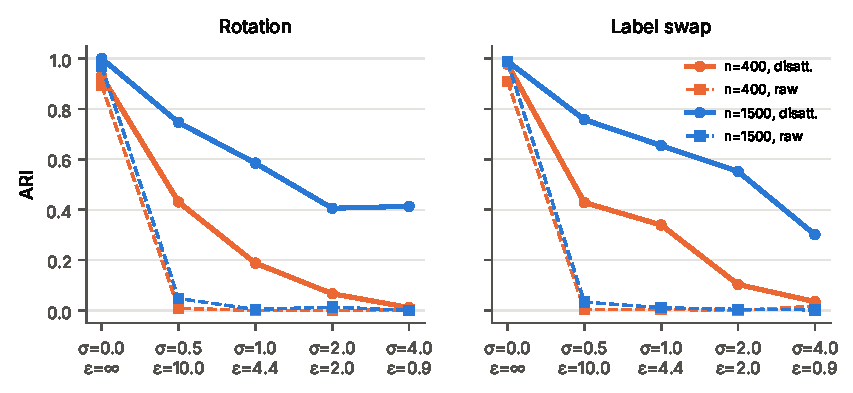
\includegraphics[width=0.85\linewidth]{dp.pdf}
\caption{Clustering quality under $(\varepsilon,10^{-5})$-DP signatures (3 seeds). Solid: DisCo-CFL; dashed: raw cosine. Orange: 400 samples per client; blue: 1{,}500.}\label{fig:dp}
\end{figure}

\paragraph{Class support.} The signatures reveal which classes a client holds (Section~\ref{sec:method}). Table~\ref{tab:support} (Appendix~\ref{app:more}) evaluates padding: under DP noise, every client also sends, for each class it does not hold, two independent noise vectors with the noise scale of its median class. Without padding the server knows the support exactly from the list of reported classes; even from the reliabilities alone ($R_i^c>0$) it would infer it with 77--92\% accuracy. With padding the list no longer reveals the support, but the reliabilities still do, with 63--84\% accuracy: a noise vector has a positive split-half correlation by chance in about 37\% of the cases, whereas a held class with enough data has a clearly positive one. Padding also costs clustering quality (ARI falls by up to $0.3$), because the noise classes add spurious evidence. It is therefore a weak mitigation. Hiding the support would need a mechanism that releases the support itself under DP, which we leave open.



\subsection{Calibration, sensitivity, ablation and cost}\label{sec:sens-cost}
\paragraph{Calibration and threshold (H3).}\label{sec:sens} Figure~\ref{fig:tau} varies $\tau$ on the clustering step. With disattenuation, ARI is $0.85$--$1.00$ for $\tau\in[0.85,0.95]$ in every concept-shift scenario, and the label-only scenario keeps $K=1$ up to $\tau=0.9$. With the raw cosine the useful range is narrower and higher thresholds over-split: at $\tau=0.95$ the label-only federation is split into 3 clusters and \emph{Rotation + QS} into 9.7 on average. Disattenuation therefore makes the threshold less sensitive towards high values, as H3 states. Towards low values the picture is reversed: at $\tau=0.8$ the raw cosine merges fewer groups than the disattenuated similarity (ARI $0.70$ against $0.60$ on \emph{Rotation}), because disattenuation raises all similarities, including those between groups. A calibrated scale thus shifts the useful range of $\tau$ upwards rather than widening it on both sides. The gain at the default threshold is moderate: without disattenuation (Table~\ref{tab:abl}) ARI drops by $0.04$--$0.11$ in the concept-shift scenarios and by $0.33$ in the label-only one. The sample-size study (Figure~\ref{fig:size} in Appendix~\ref{app:figs}) shows why. With clipped per-sample gradients, the raw cosine between clients of the same group is already $0.98$ on Fashion-MNIST, so there is little attenuation to correct; the disattenuated similarity is $0.99$--$1.00$. Attenuation becomes large under DP noise, where the raw cosine fails completely (Figure~\ref{fig:dp}). With very small clients (50--100 samples) both versions fail, for another reason: the groups become close at the reference model (between-group similarity $0.89$--$0.93$), i.e.\ the separation shrinks, and disattenuation does not help (ARI $0.13$--$0.63$, against $0.21$--$0.60$ for the raw cosine). Otsu's label-free threshold (Table~\ref{tab:diag}) lies at $0.76$--$0.83$ in the concept-shift scenarios. It recovers label swaps as well as $\tau=0.9$ (ARI $0.97$) but merges groups under rotations (ARI $0.58$--$0.71$). Over all scenarios (Table~\ref{tab:diag}) the comparison is two-sided. In the seven scenarios where DisCo-CFL fails (ARI below $0.5$), Otsu's threshold is better in four (e.g.\ Office-Home, $0.70$ against $0.26$; CIFAR-10 rotations with the pretrained network, $0.50$ against $0.07$), equal in the two SVHN scenarios and worse in one. In the 24 scenarios where DisCo-CFL succeeds it is lower in 19, equal in four and higher in one, and it splits single-concept federations (ARI $0$ in the label-only scenario). Its separation index $\eta$ does not distinguish successes from failures ($0.63$ for the $45^\circ$ rotation with ARI $1.00$, $0.73$ for CIFAR-10 label swaps with ARI $0.28$), so neither threshold dominates, and Otsu's rule does not replace $\tau$. The shrinkage $\lambda$ has almost no effect between $0.02$ and $1$ (Table~\ref{tab:lambda} in Appendix~\ref{app:figs}), including the values $0.02$ and $0.1$ that satisfy the condition of Corollary~\ref{cor:sc}.

\begin{figure}[!htbp]
\centering
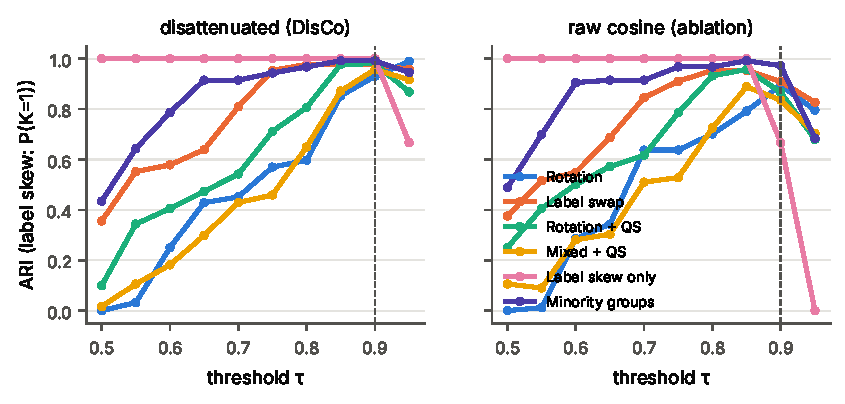
\includegraphics[width=0.85\linewidth]{tau_sensitivity.pdf}
\caption{Sensitivity to the threshold $\tau$ (3 seeds). The dashed line marks the default $\tau=0.9$, selected on the pilot runs (Section~\ref{sec:setup}).}\label{fig:tau}
\end{figure}

\paragraph{Edge cases.} The edge-case rules of Section~\ref{sec:method} were evaluated in three federations (Table~\ref{tab:edge} in Appendix~\ref{app:more}): the default minimum class size $m=4$ is best or close to best, the reliability floor $r_{\min}$ has no measurable effect, and extreme label skew ($\alpha=0.1$) or small clients lower ARI to about $0.7$.

\paragraph{Ablation (H3, H4).}
Table~\ref{tab:abl} removes one component at a time. Without class conditioning (one signature per client over all its data), clients are grouped by their label mix, the failure mode reported in the survey~\citep{benali2026survey}: 18--33 clusters and a concept accuracy 19 points lower. The mean linkage averages class-specific shifts away and merges conflicting clients (11.3\% on average, ARI $0.48$ under rotations), which supports H4: the minimum over classes matters. Linkage-ordered merging over-splits label swaps and \emph{Mixed + QS}. Without disattenuation or without clipping the federation is split more often, most visibly in the label-only scenario. Without the attachment stage, a noisy client stays alone in the label-only scenario in one of the three seeds. The table uses seeds 0--2 for all rows, so the DisCo-CFL row differs slightly from the five-seed means of Table~\ref{tab:main}. The ablation supports class conditioning and the bottleneck linkage clearly; evidence-ordered merging and clipping matter only in some scenarios (linkage-ordered merging is slightly better on \emph{Rotation}), and these two choices rest mainly on the pilot runs.

\begin{tableorg}[!htbp]
\centering
\caption{Ablation (Fashion-MNIST, 3 seeds): ARI / number of clusters $K$ per scenario, mean conflict-merge rate (\%) and mean concept accuracy (\%) over the five scenarios.}\label{tab:abl}
\scriptsize
\setlength{\tabcolsep}{3pt}
\resizebox{\textwidth}{!}{%
\begin{tabular}{lccccccc}
\toprule
Variant & Rotation & Label swap & Rot.\,+\,QS & Mixed\,+\,QS & Label only & Conflict\% & Concept \\
\midrule
DisCo-CFL (full) & 0.93 / 4.3 & 0.98 / 4.0 & 0.98 / 4.3 & 0.96 / 4.0 & 1.00 / 1.0 & 0.2 & 76.9 \\
without disattenuation (raw cosine) & 0.89 / 5.0 & 0.91 / 4.7 & 0.87 / 5.3 & 0.86 / 5.0 & 0.67 / 1.3 & 0.4 & 76.0 \\
without class conditioning & 0.05 / 31.7 & 0.04 / 32.7 & 0.03 / 33.0 & 0.02 / 29.0 & 0.00 / 17.7 & 0.8 & 57.9 \\
mean instead of bottleneck linkage & 0.48 / 3.0 & 0.70 / 4.0 & 0.79 / 4.0 & 0.58 / 4.0 & 1.00 / 1.0 & 11.3 & 73.6 \\
linkage-ordered merging & 0.95 / 4.7 & 0.85 / 5.3 & 0.97 / 4.3 & 0.77 / 6.3 & 0.67 / 1.3 & 0.0 & 75.7 \\
without per-sample clipping & 0.93 / 4.3 & 1.00 / 4.0 & 0.93 / 5.0 & 0.93 / 4.3 & 0.33 / 1.7 & 0.2 & 76.6 \\
without attachment stage & 0.91 / 5.0 & 0.98 / 4.0 & 0.97 / 4.7 & 0.96 / 4.0 & 0.67 / 1.3 & 0.1 & 76.7 \\
\bottomrule
\end{tabular}}
\end{tableorg}

\paragraph{Cost and scalability.}\label{sec:cost}
Table~\ref{tab:cost} reports wall-clock time per run and the floats each client uploads for clustering. Each DisCo-CFL client uploads its signature \emph{once}, $2p|S_i|\le2pC\approx2.0\times10^4$ floats with $p=1024$ ($1.8$--$2.0\times10^4$ on average for the default configuration in Table~\ref{tab:cost}), independent of the model dimension $d$ (46{,}730 for the small CNN, 8.4M for the ResNet-18 block). FL+HC and StoCFL upload $d$-dimensional updates or gradients for clustering, IFCA downloads $K$ models per client in every round, and FedCCFA exchanges classifiers and class anchors in every round. A DisCo-CFL run takes about as long as a FedAvg run (the times come from shared machines, so differences below about 20\% are noise; FedAvg-FT appears faster than FedAvg on the realistic benchmarks for this reason); StoCFL takes about twice as long because it trains two models per round. Computing the signature takes about 0.09\,s per client on one CPU core, and server-side clustering 0.09\,s for 40 clients and 6\,s for 320 clients. In the clustering-only scalability study, which uses 200 samples per client, ARI is $0.59$--$0.82$ for 40 to 320 clients. With 200 clients in the full pipeline (Table~\ref{tab:sweeps}) ARI is $0.88$ and accuracy is within $0.7$ points of the Oracle. The scalability study uses one seed per size and its ARI is not monotone in the number of clients, so it measures time rather than recovery.

\begin{tableorg}[!htbp]
\centering
\caption{Cost per run: mean wall-clock time (minutes; one CPU core for the small CNN, one GPU for the realistic benchmarks) and floats uploaded per client for the clustering signal. DisCo-AS: label-free warm-up (Section~\ref{sec:warmup}); DisCo-full: signature from the gradient of the whole layer-4 block (realistic benchmarks); DisCo-linkorder, DisCo-mean, DisCo-noClass, DisCo-noClip and DisCo-noDisatt: the ablation variants of Table~\ref{tab:abl} (linkage-ordered merging, mean linkage, without class conditioning, without clipping, without disattenuation).}\label{tab:cost}
{\scriptsize
\resizebox{\textwidth}{!}{%
\begin{tabular}{l c c c}
\toprule
Method & Time, small-CNN main (min) & Time, realistic (min) & Upload floats / client \\
\midrule
DisCo & 6.9 & 0.8 & 1.9e4 \\
DisCo-noAttach & 6.9 & 0.8 & 2.0e4 \\
DisCo-T30 & -- & 1.2 & 1.9e4 \\
FedAvg & 7.1 & 1.4 & 0 \\
Local & 6.9 & 1.4 & 0 \\
FedAvg-FT & 7.6 & 0.7 & 0 \\
IFCA & 11.0 & 2.6 & 0 \\
FeSEM & 7.7 & 1.5 & 0 \\
MTCFL & 6.1 & 0.8 & 0 \\
FL+HC & 7.6 & 1.6 & 2.0e6 \\
PACFL & 7.5 & 1.5 & 3.3e3 \\
StoCFL & 13.9 & 3.1 & 2.0e6 \\
StoCFL-W & 12.5 & 1.7 & 2.0e6 \\
FedCCFA & 5.2 & 5.8 & 5.9e5 \\
FedDAG-C & 7.9 & 1.5 & 5.8e4 \\
Oracle & 7.2 & 1.4 & 0 \\
DisCo-AS & 7.2 & -- & 1.5e4 \\
DisCo-full & -- & 1.8 & 3.7e4 \\
DisCo-linkorder & 6.3 & 1.1 & 1.8e4 \\
DisCo-mean & 6.0 & 1.2 & 1.8e4 \\
DisCo-noClass & 6.0 & 1.1 & 2.0e3 \\
DisCo-noClip & 5.9 & 1.2 & 1.8e4 \\
DisCo-noDisatt & 6.0 & 1.1 & 1.8e4 \\
\bottomrule
\end{tabular}}
}

\end{tableorg}

